\documentclass[10pt]{article}
\usepackage[ngerman]{babel}
\usepackage[utf8]{inputenc}
\usepackage[T1]{fontenc}
\usepackage{graphicx}
\usepackage[export]{adjustbox}
\graphicspath{ {./images/} }
\usepackage{amsmath}
\usepackage{amsfonts}
\usepackage{amssymb}
\usepackage[version=4]{mhchem}
\usepackage{stmaryrd}

\title{Bachelor of Science (BSc) in Informatik Modul Software-Entwicklung 1 (SWEN1) }

\author{}
\date{}


\begin{document}
\maketitle
\section*{LE 07 - Use Case Realization Zusammenfassung}
SWEN1/PM3 Team:\\
R. Ferri (feit), D. Liebhart (lieh), K. Bleisch (bles), G. Wyder (wydg)

\section*{Um was geht es?}
\begin{itemize}
  \item Wie kann ich aus den Analyse- und Design-Artefakten die eigentliche Realisierung der Use-Cases machen?
  \item Wie wende ich GRASP Patterns korrekt an?
  \item Wie komme ich schlussendlich zu lauffähigem und korrektem Code?
\end{itemize}

\section*{Lernziele LE 07 - Use Case Realization}
\begin{itemize}
  \item Sie sind in der Lage:
  \item Use Cases zu realisieren, was Sie mit UML-Artefakten dokumentieren
  \item den Quellcode aus den Design Artefakten abzuleiten
\end{itemize}

\begin{enumerate}
  \item Einfluss Analyse Artefakte
  \item UML und Design to Code
  \item Repetition GRASP
  \item Vorgehen
  \item Fallstudie «NextGenPos»
  \item Fallstudie «Monopoly»
  \item Wrap-up und Ausblick
\end{enumerate}

\section*{Denkpause}
\section*{Aufgabe 7.1 (5’)}
Wir haben in den LE02 - LE04 verschieden Artefakte kennengelernt, um Anforderungen zu spezifizieren. Dazu gehören:

\begin{itemize}
  \item Use Cases
  \item System-Sequenzdiagramm (SSD)
  \item Operation Contract (Systemverträge)
  \item Domänenmodell
\end{itemize}

Repetieren Sie, zuerst ohne nachzuschlagen, den Aufbau und die Varianten dieser Artefakte. Schätzen Sie ab, welche Information daraus für die Realisierung von grossem Nutzen sind.

\section*{Analyse Artefakte und Use-Case-Realization}
School of\\
Engineering\\
InIT Institut für angewandte Informationstechnologie\\
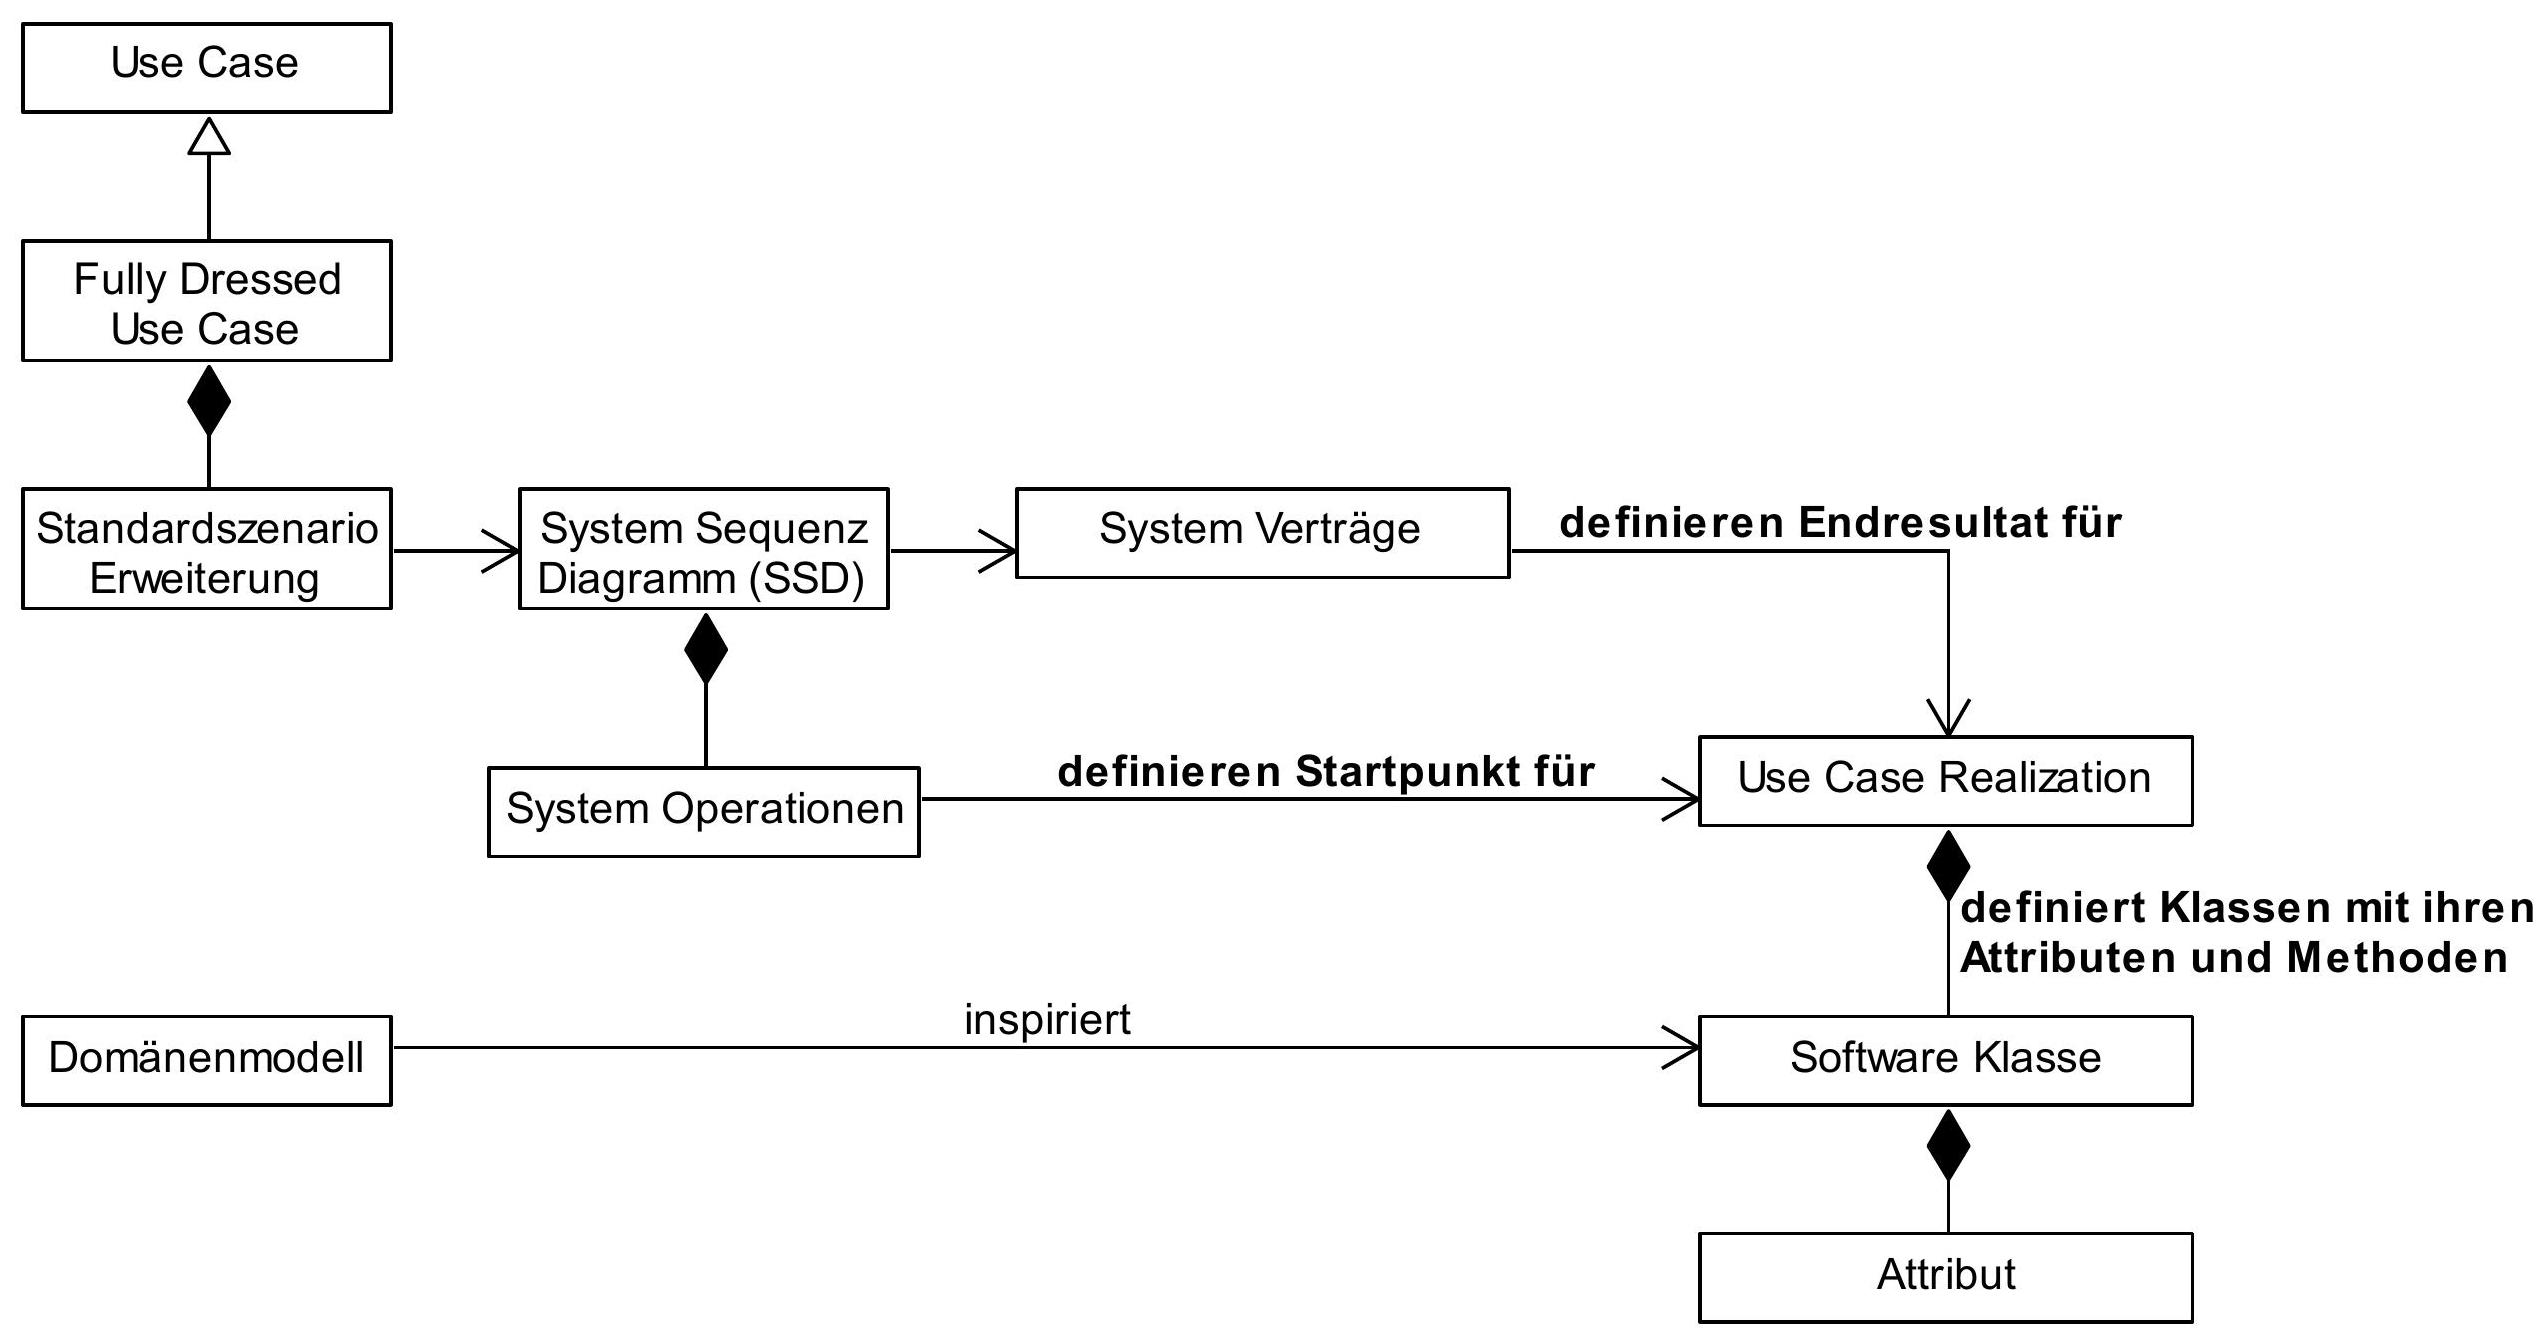
\includegraphics[width=\linewidth]{images/2025_01_02_1fd681d207513c8e8344g-06}

\begin{enumerate}
  \item Einfluss Analyse Artefakte
  \item UML und Design to Code
  \item Repetition GRASP
  \item Vorgehen
  \item Fallstudie «NextGenPos»
  \item Fallstudie «Monopoly»
  \item Wrap-up und Ausblick
\end{enumerate}

\begin{itemize}
  \item Das zu erreichende Ziel der Use-Case-Realization ist der lauffähige und korrekte Code.
  \item UML (Klassendiagramm, Interaktionsdiagramme) kann dafür als Zwischenschritt verwendet werden.
  \item Empfehlenswert für alle, die noch wenig Erfahrung in der Software Entwicklung haben.
  \item Hängt von den Vorgaben der Organisation ab, in der man tätig ist.
  \item In diesem Modul, und speziell in dieser Lerneinheit, wird UML als Ersatz für eine Programmiersprache aus didaktischen Gründen verwendet.
  \item Keine Details der Programmiersprache, die den Lerninhalt «vernebeln».
  \item Zusammenarbeit der Klassen ist klarer sichtbar.
  \item Kompaktere Darstellung der wesentlichen Aspekte.
\end{itemize}

\section*{Warum UML? (2/2)}
\begin{itemize}
  \item Für eine nicht beteiligte Person ist UML einfacher zu verstehen als der reine Code.
  \item In der Praxis, insbesondere bei agilen Methoden, wird auf eine vollständige Dokumentation mit UML verzichtet.
  \item Es kann aber gut möglich sein, dass die Organisation, für die Sie arbeiten, gewisse Dokumentationsvorgaben stellt. In diesem Fall ist der Einsatz von UML zu prüfen.
\end{itemize}

\section*{Übersicht Design -> Code}
Welche Informationen können Sie aus den Design Artefakten für die eigentliche Implementierung ableiten? Und in welchem Detaillierungsgrad?

Design Artefakte\\
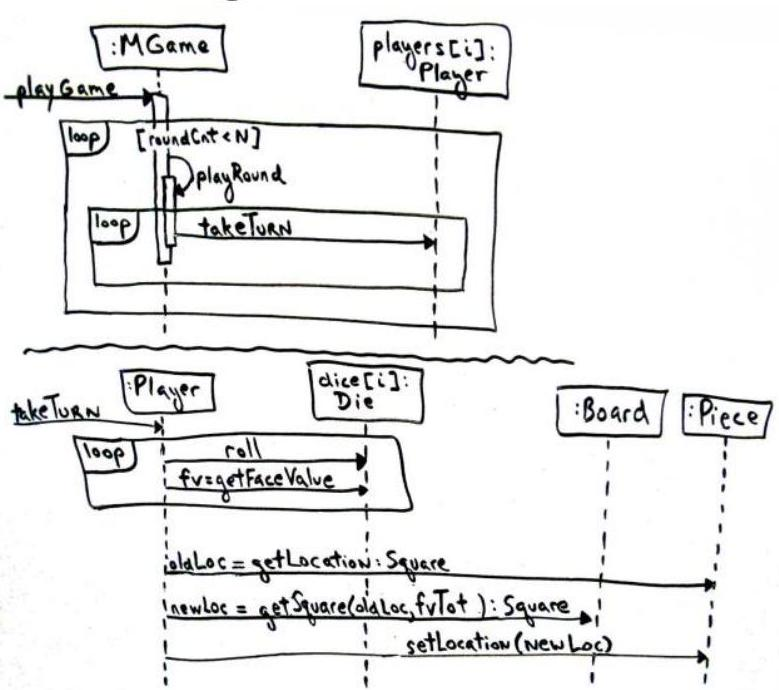
\includegraphics[width=\linewidth]{images/2025_01_02_1fd681d207513c8e8344g-10}

Ausführbarer Code\\
public class MonopolyGame \{\\
public void playGame()\\
int roundCnt $=0$;\\
while(roundCnt < 1000)\{\\
PlayRound()\\
\}\\
\}\\
private void playRound()\{\\
// ...•\\
\}

\section*{Beispiel Fallstudie: NextGenPos DCD - Design Class Diagramm}
School of Engineering\\
InIT Institut für angewandte Informationstechnologie

\begin{itemize}
  \item Klassen
  \item Attribute
  \item Methoden
  \item Assoziation\\
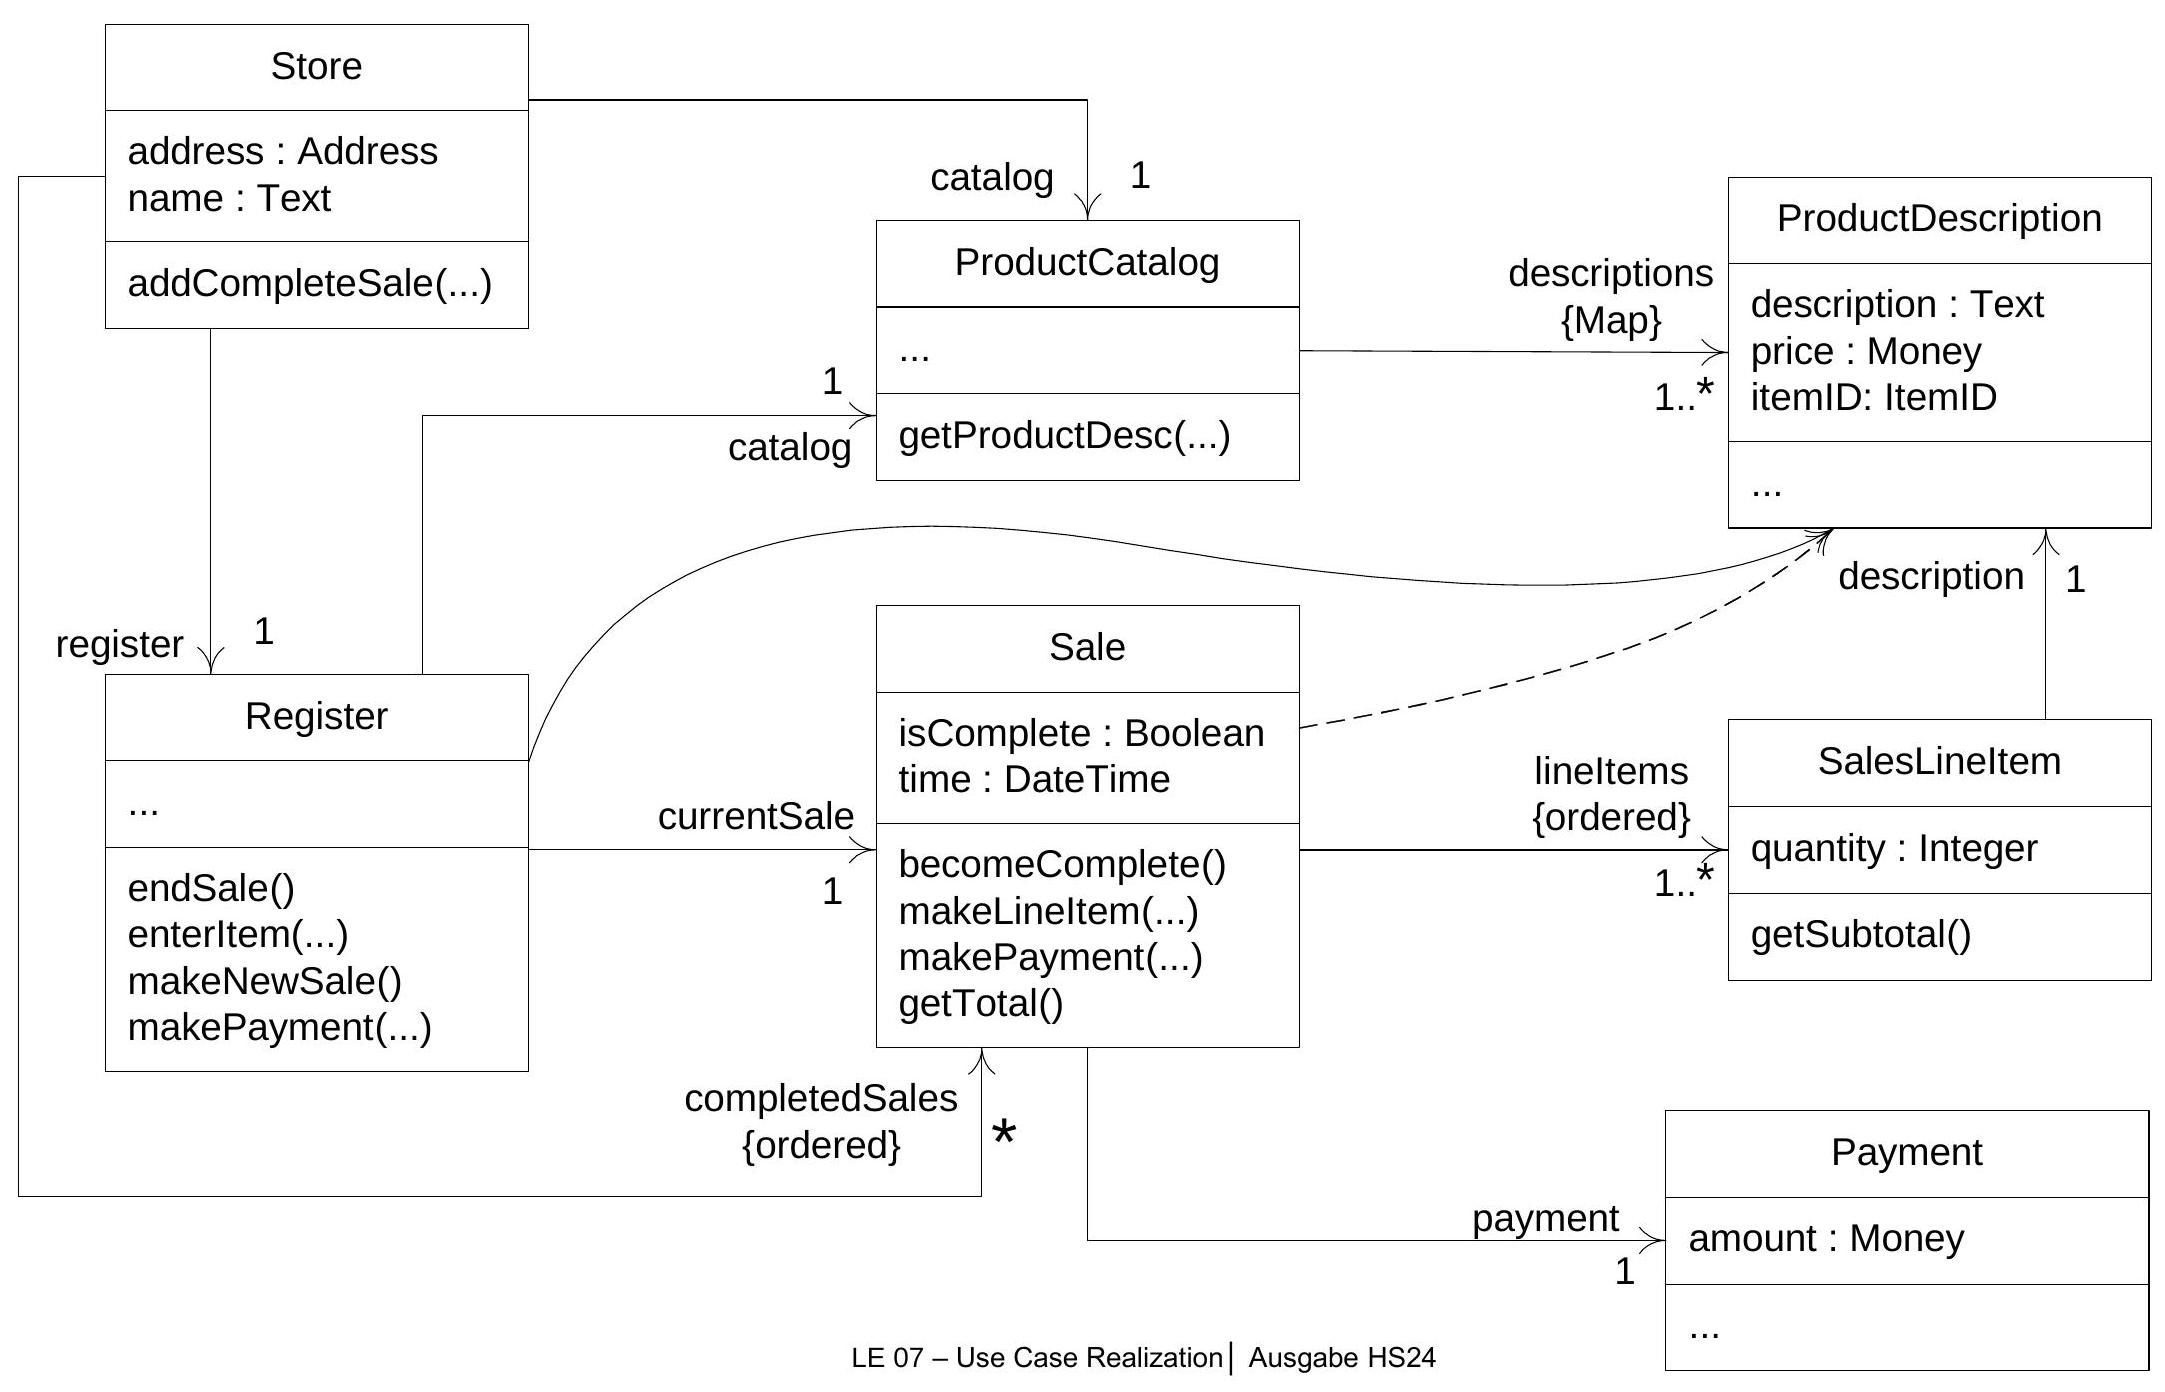
\includegraphics[width=\linewidth]{images/2025_01_02_1fd681d207513c8e8344g-11}
\end{itemize}

\section*{Beispiel Fallstudie: NextGenPos Methoden aus Interaktionsdiagrammen}
\begin{itemize}
  \item Methoden mit Signaturen\\
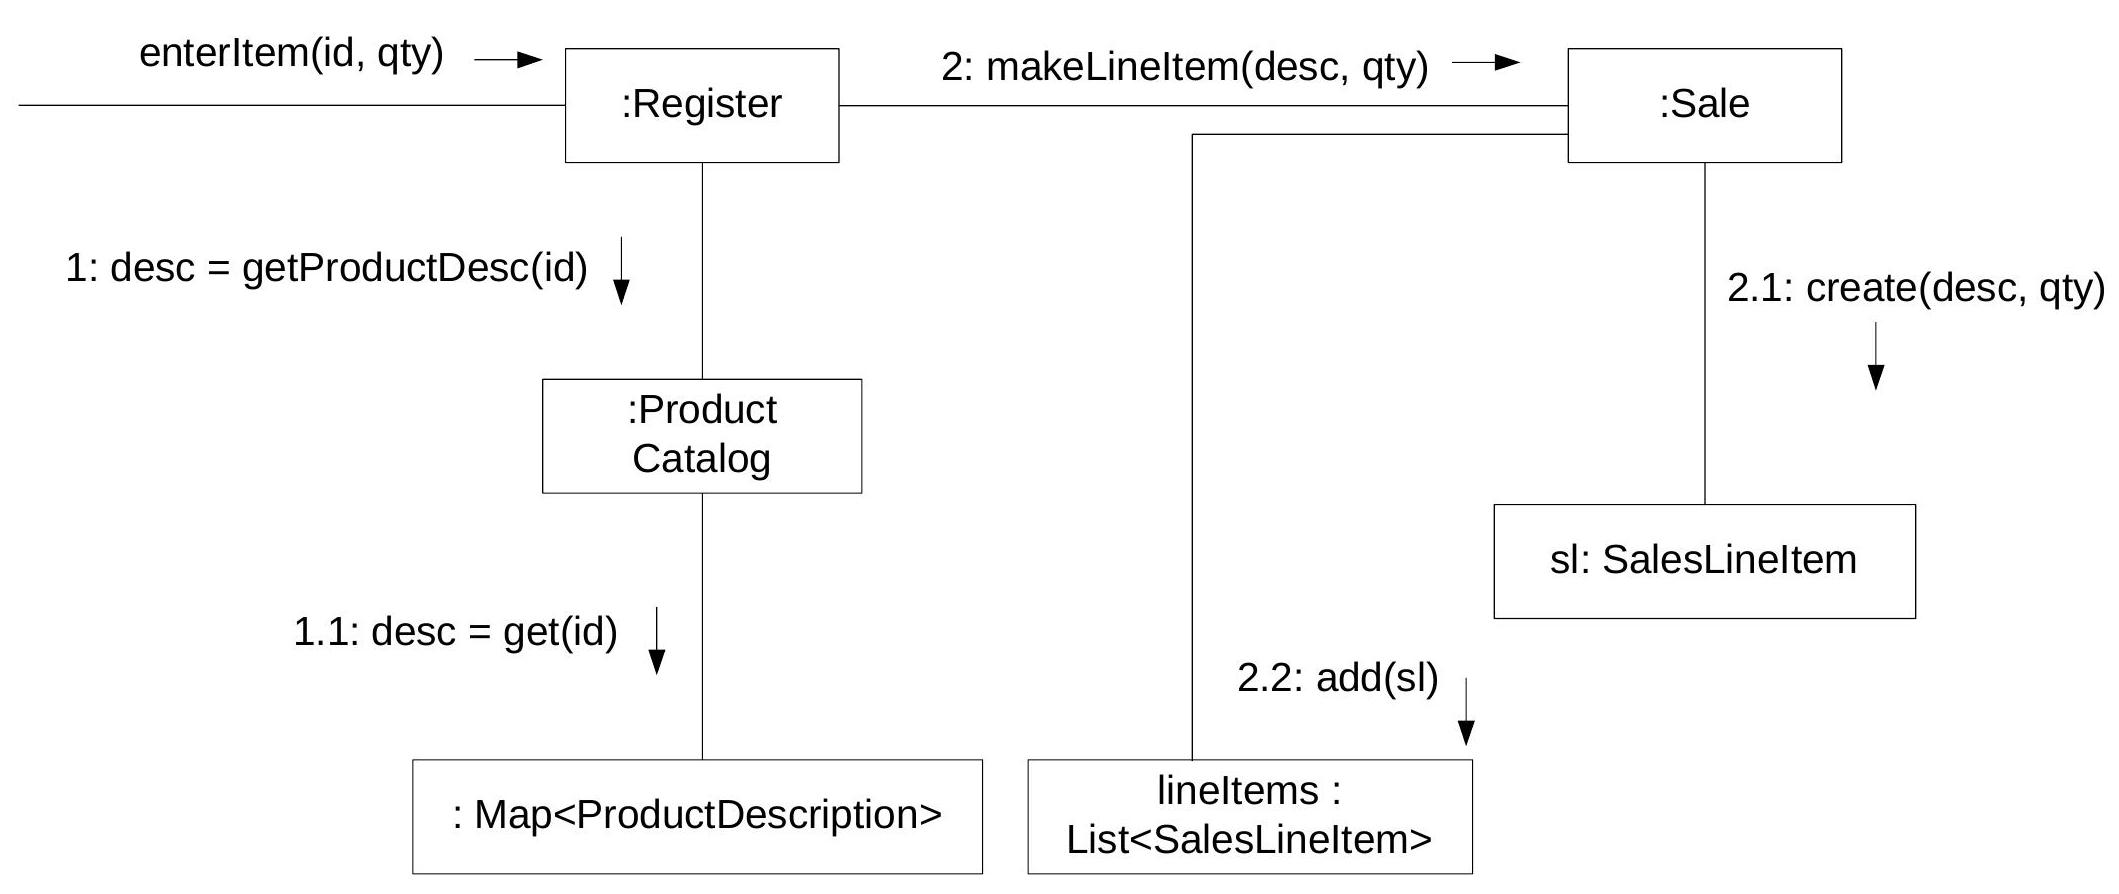
\includegraphics[width=\linewidth]{images/2025_01_02_1fd681d207513c8e8344g-12}
\end{itemize}

Register.enterItem(int itemId, int qty);\\
// Zwei Ereignisse werden an sichtbare Klassen gesendet\\
ProductDesription desc = catalog.getProductDescription(itemId); currentSale.makeLineItem(desc, qty);

\begin{enumerate}
  \item Einfluss Analyse Artefakte
  \item UML und Design to Code
  \item Repetition GRASP
  \item Vorgehen
  \item Fallstudie «NextGenPos»
  \item Fallstudie «Monopoly»
  \item Wrap-up und Ausblick
\end{enumerate}

\section*{Denkpause}
\section*{Aufgabe 7.2 (5')}
Wir haben in den LE06 die GRASP Prinzipien kennengelernt für ein gutes, objektorientiertes Design:

\begin{itemize}
  \item Information Expert
  \item Creator
  \item Controller
  \item Low Coupling
  \item High Cohesion
  \item Polymorphism
  \item Pure Fabrication
  \item Indirection
  \item Protected Variations
\end{itemize}

Repetieren Sie, zuerst ohne nachzuschlagen, diese Prinzipien.

\section*{GRASP - Die 5 wichtigsten Prinzipien}
Für die Use-Case-Realization sind insbesondere die 5 ersten Prinzipien zentral:

\begin{itemize}
  \item Information Expert
  \item Eine Klasse bekommt die Verantwortlichkeit, wofür sie die notwendigen Informationen hat
  \item Creator
  \item 3 Regeln, um die Erzeugung einer Instanz einer Klasse zuzuweisen
  \item Controller
  \item Der Fassaden-Controller übernimmt als erste Instanz vom UI die Ausführung der Systemoperationen
  \item Low Coupling
  \item Bei mehreren Varianten ist die zu bevorzugen, die weniger Kopplungen hat
  \item High Cohesion
  \item Die Verantwortlichkeiten einer Klasse sollten möglichst kohäsiv («fokussiert») sein.
\end{itemize}

\begin{enumerate}
  \item Einfluss Analyse Artefakte
  \item UML und Design to Code
  \item Repetition GRASP
  \item Vorgehen
  \item Fallstudie «NextGenPos»
  \item Fallstudie «Monopoly»
  \item Wrap-up und Ausblick
\end{enumerate}

\section*{Vorbereitung}
\begin{enumerate}
  \item Use Case auswählen, offene Fragen klären, SSD ableiten
  \item Systemoperation auswählen
  \item Operation Contract (Systemvertrag) für diese Systemoperation erstellen/überlegen/lesen
  \item Aktueller Code/Dokumentation des relevanten Teils der Software analysieren.
  \item DCD überprüfen/aktualisieren
  \item Vergleich mit relevantem Teil des Domänenmodells durchführen
  \item Allenfalls bereits jetzt neue Software Klassen erstellen gemäss Vorlage Domänenmodell
  \item Falls notwendig, Refactorings durchführen
\end{enumerate}

\section*{Vorgehen}
\begin{enumerate}
  \item Controller Klasse bestimmen resp. identifizieren
\end{enumerate}

\begin{itemize}
  \item Siehe GRASP Controller Pattern
\end{itemize}

\begin{enumerate}
  \setcounter{enumi}{1}
  \item Zu verändernde Klassen festlegen
  \item Weg zu diesen Klassen festlegen
\end{enumerate}

\begin{itemize}
  \item Allenfalls mit Hilfe von Parametern den richtigen Weg auswählen
  \item Allenfalls Klassen, die notwendig sind, neu erstellen
  \item Immer Aufruf weiterleiten mit allen noch notwendigen Parametern
  \item Verantwortlichkeiten gemäss GRASP Information Expert zuweisen
  \item In Varianten denken, Varianten gemäss Low Coupling und High Cohesion bewerten.
\end{itemize}

\begin{enumerate}
  \setcounter{enumi}{3}
  \item Veränderungen gemäss Systemvertrag programmieren
  \item Review bezüglich High Cohesion und Architekturkonformität
  \item Einfluss Analyse Artefakte
  \item UML und Design to Code
  \item Repetition GRASP
  \item Vorgehen
  \item Fallstudie «NextGenPos»
  \item Fallstudie «Monopoly»
  \item Wrap-up und Ausblick
\end{enumerate}

\begin{itemize}
  \item Wir führen nun die Use-Case Realization von UC Process Sale des Projekts NextGenPos durch. Es ist das Fallbeispiel aus Larman[1]
  \item makeNewSale()
  \item enterItem(idemId, quantity)
  \item endSale()
  \item getTotal()
  \item makePayment()
  \item UML nochmal kurz erwähnt:
  \item Es folgen sehr viele UML-Artefakte und schriftliche Erklärungen.
  \item Dies geschieht aus didaktischen Gründen.
  \item Die Überlegungen dahinter sollten Sie auf alle Fälle machen.
  \item Wieviel UML in der Praxis gezeichnet wird, ist eine Frage, die wir bereits erörtert haben.
\end{itemize}

\section*{Analyse Artefakte: Domänenmodell}
School of\\
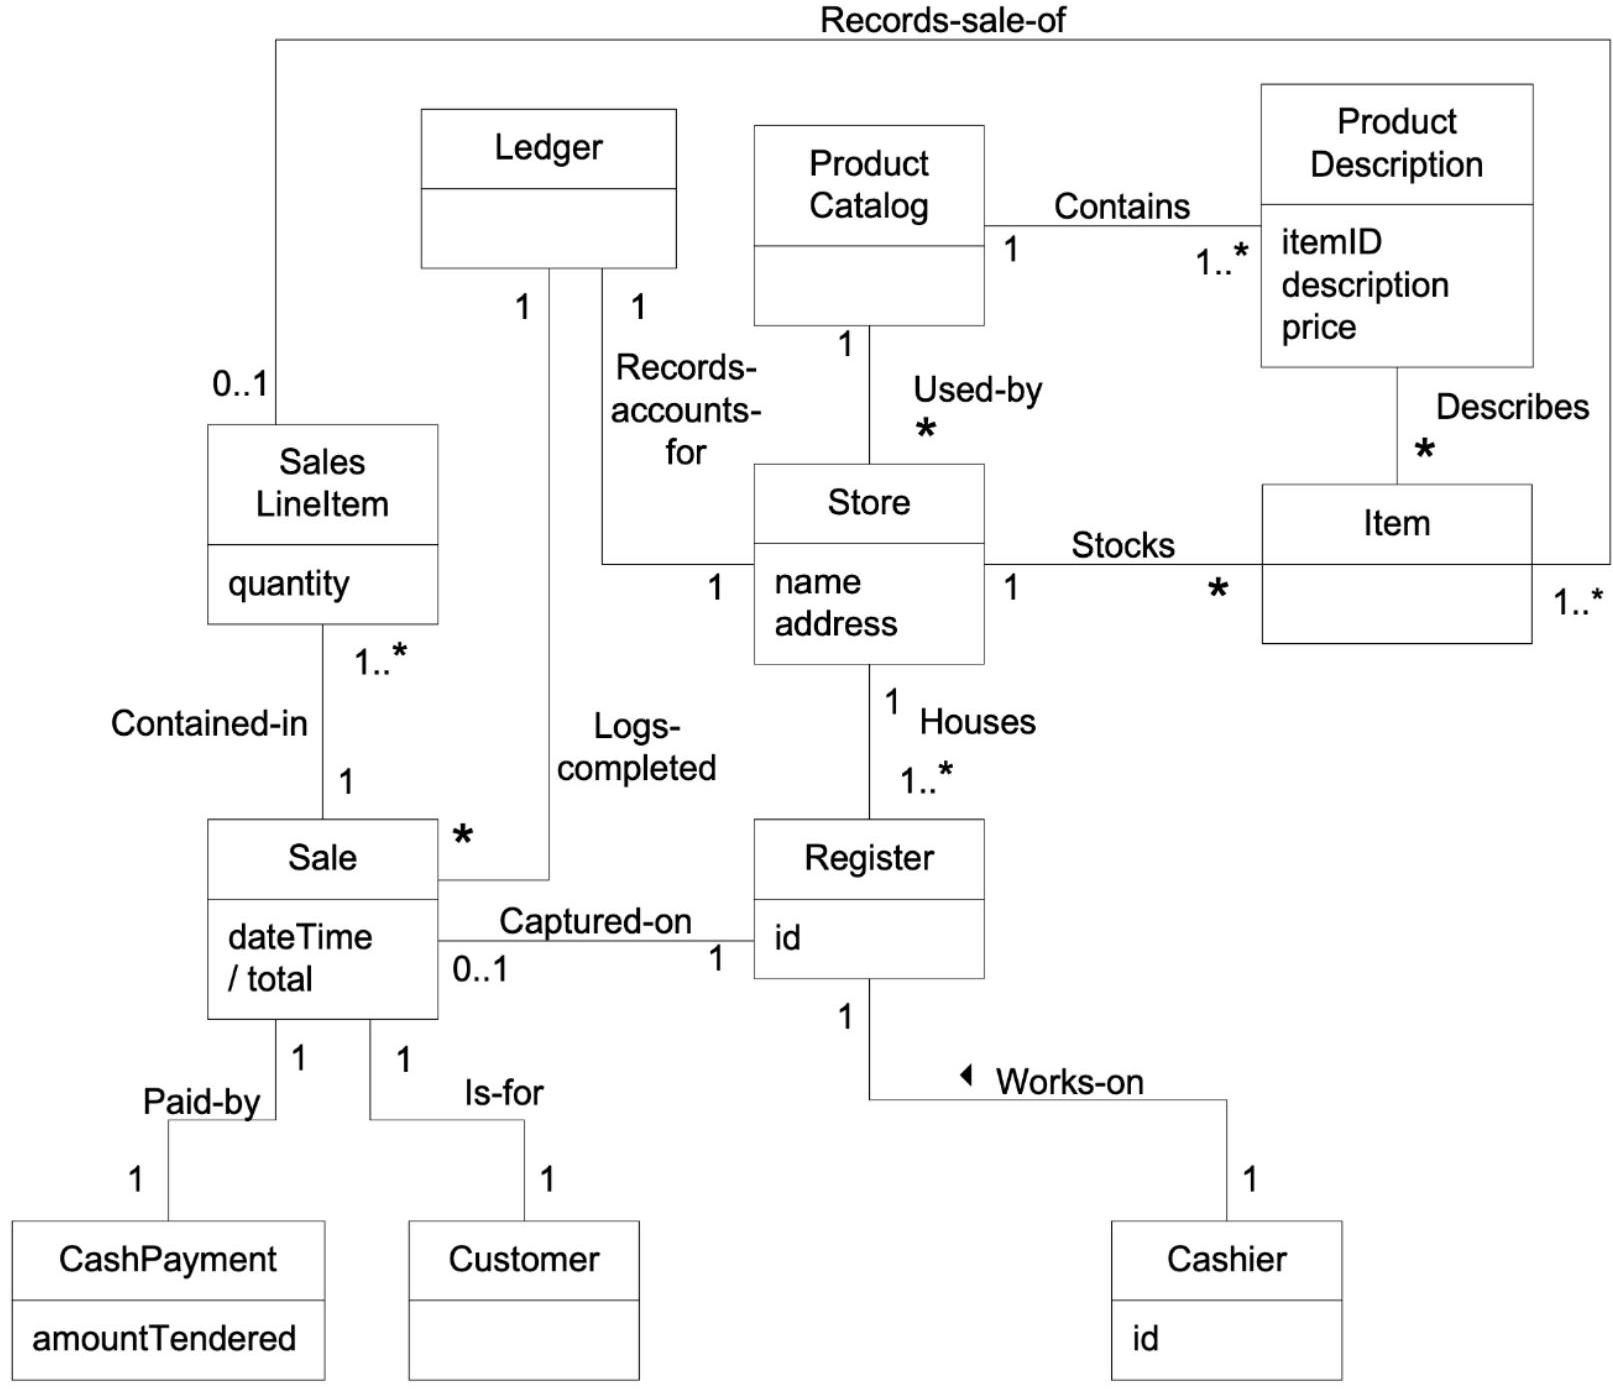
\includegraphics[width=\linewidth]{images/2025_01_02_1fd681d207513c8e8344g-21}

\section*{Analyse Artefakte: Use Case und SSD}
\section*{Use Case, Standardszenario}
Simple cash-only Process Sale scenario:

\begin{enumerate}
  \item Customer arrives at a POS checkout with goods and/or services to purchase.
  \item Cashier starts a new sale.
  \item Cashier enters item identifier.
  \item System records sale line item and presents item description, price, and running total.
\end{enumerate}

Cashier repeats steps 3-4 until indicates done.\\
5. System presents total with taxes calculated.\\
6. Cashier tells Customer the total and asks for payment.\\
7. Customer pays and System handles payment.

System Sequenz Diagramm\\
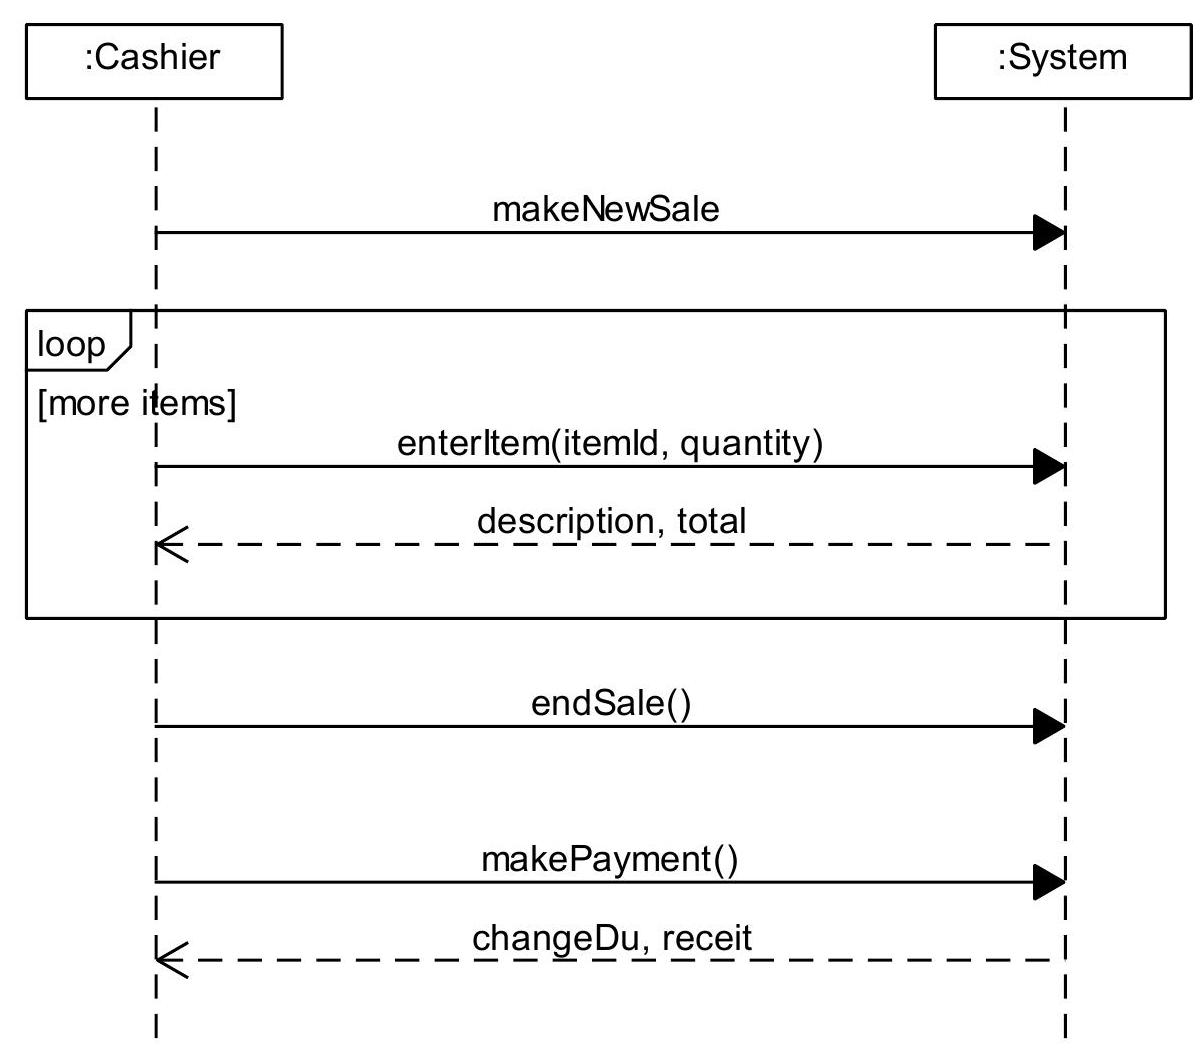
\includegraphics[width=\linewidth]{images/2025_01_02_1fd681d207513c8e8344g-22}

\section*{makeNewSale (1)}
\section*{- Vorbereitungsarbeiten}
\begin{enumerate}
  \item Use Case «Process Sale», fully dressed ausgearbeitet
  \item Systemoperation «makeNewSale()
  \item Operation Contract, Nachbedingungen
\end{enumerate}

\begin{itemize}
  \item Neue Sale-Instanz s ist erstellt
  \item S ist die neue aktuelle Sale Instanz von Register
\end{itemize}

\begin{enumerate}
  \setcounter{enumi}{3}
  \item Aktueller Status der Software: Erste Systemoperation überhaupt, noch nichts erstellt
  \item Klassen Register und Sale gemäss DM erstellen\\
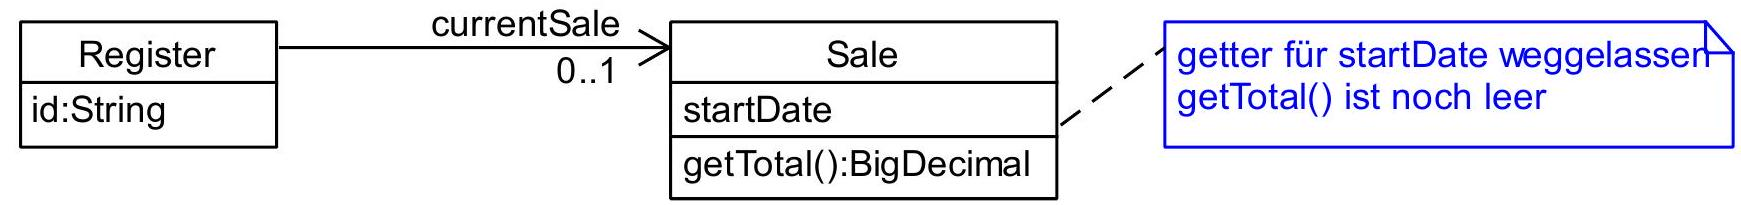
\includegraphics[width=\linewidth]{images/2025_01_02_1fd681d207513c8e8344g-23}
\end{enumerate}

\begin{itemize}
  \item Controller Klasse bestimmen: GRASP, Controller Pattern anwenden
  \item Für kleine Anwendungen reicht ein Fassaden Controller, der normalerweise das System darstellt, das neu entwickelt wird
  \item Register ist das System, daher wird die SW-Klasse die Controller Klasse
  \item Veränderungen festlegen
  \item Neue Instanz von Sale erstellen
  \item Diese als neue aktuelle Sale Instanz in Register ablegen
  \item Weg zum Ziel festlegen: Register ist bereits der Controller, wir brauchen keine Zwischenschritte.
  \item Sale wird erzeugt: Creator Pattern anwenden. Register ist der Container von Sale, daher soll Register eine neue Instanz von Sale erzeugen.\\
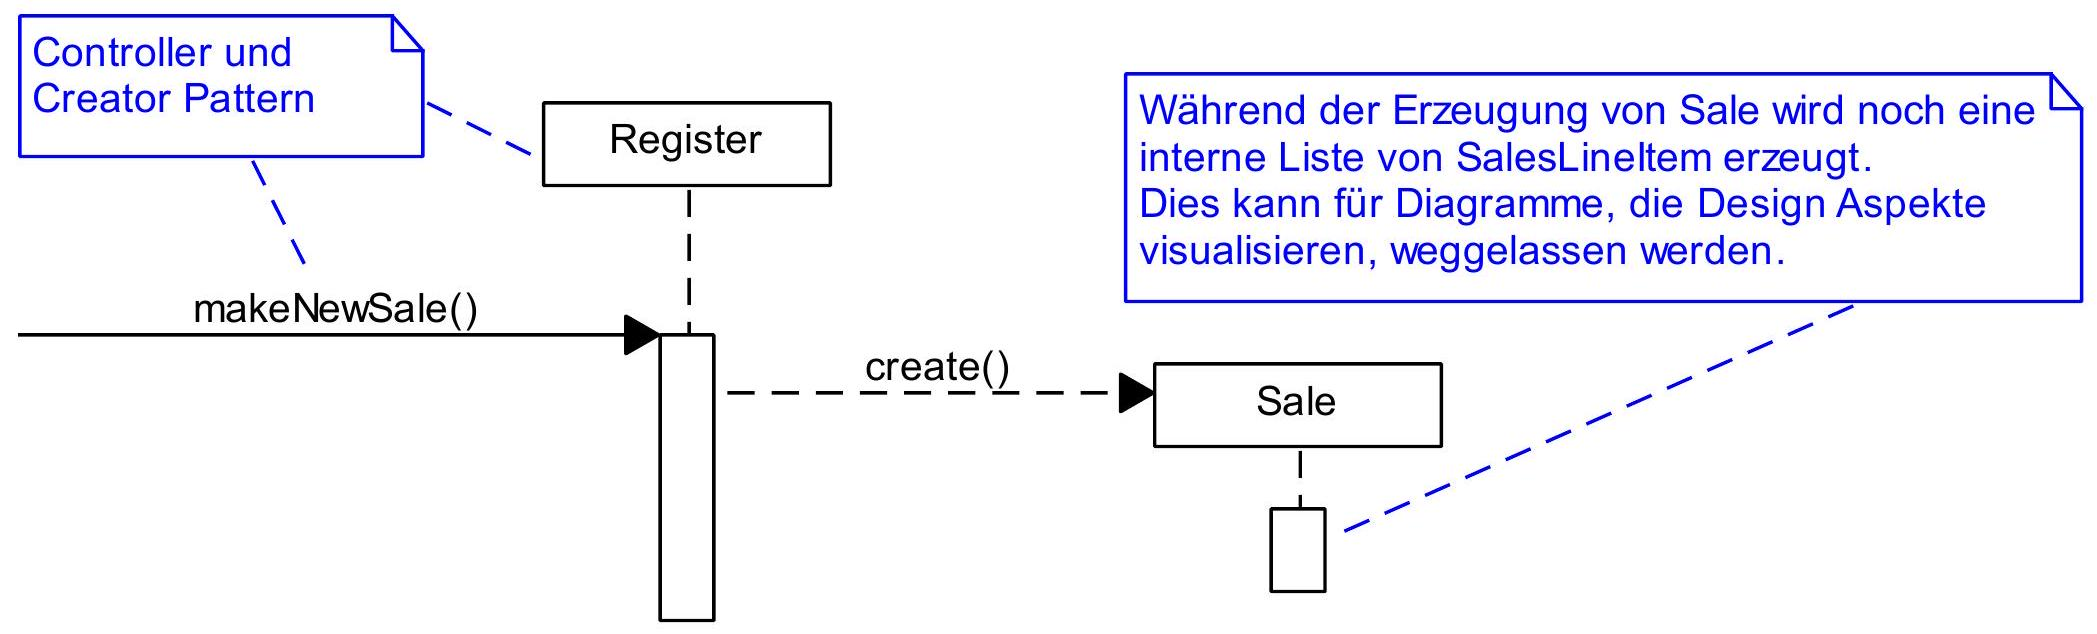
\includegraphics[width=\linewidth]{images/2025_01_02_1fd681d207513c8e8344g-25}
\end{itemize}

Review

\begin{itemize}
  \item Die Kohäsion von Register als Controller kann heikel sein, wenn dem Controller zu viel Verantwortlichkeit zugeteilt wird. Hier hat er aber Aufgaben, für die es keine andere sinnvolle Domänenklasse gibt.
  \item Das Schichten-Prinzip wurde eingehalten.
\end{itemize}

\section*{Enterltem (1)}
\section*{Vorbereitungsarbeiten}
\begin{enumerate}
  \item Use Case «Process Sale», fully dressed ausgearbeitet
  \item Systemoperation «enterltem(itemId, quantity)
  \item Operation Contract, Nachbedingungen
\end{enumerate}

\begin{itemize}
  \item SaleLineItem-Instanz sli (ist) erstellt
  \item sli mit aktueller Sale-Instanz verknüpft
  \item sli.quantity auf quantity gesetzt
  \item sli mit entsprechender ProductDescription verknüpft (gemäss itemID)
\end{itemize}

\begin{enumerate}
  \setcounter{enumi}{3}
  \item Aktueller Status der Software: Siehe vorhergehendes Beispiel
  \item Klassen Register und Sale erstellt mit wenigen Methoden
  \item Klasse ProductDescription wird im Operation Contract erwähnt und daher gemäss DM erstellt. Dort sehen wir, dass es noch einen ProductCatalog als Behälter von ProductDescriptions gibt, daher erstellen wir auch diese Klasse.
\end{enumerate}

\section*{Klassendiagramm:}
\begin{center}
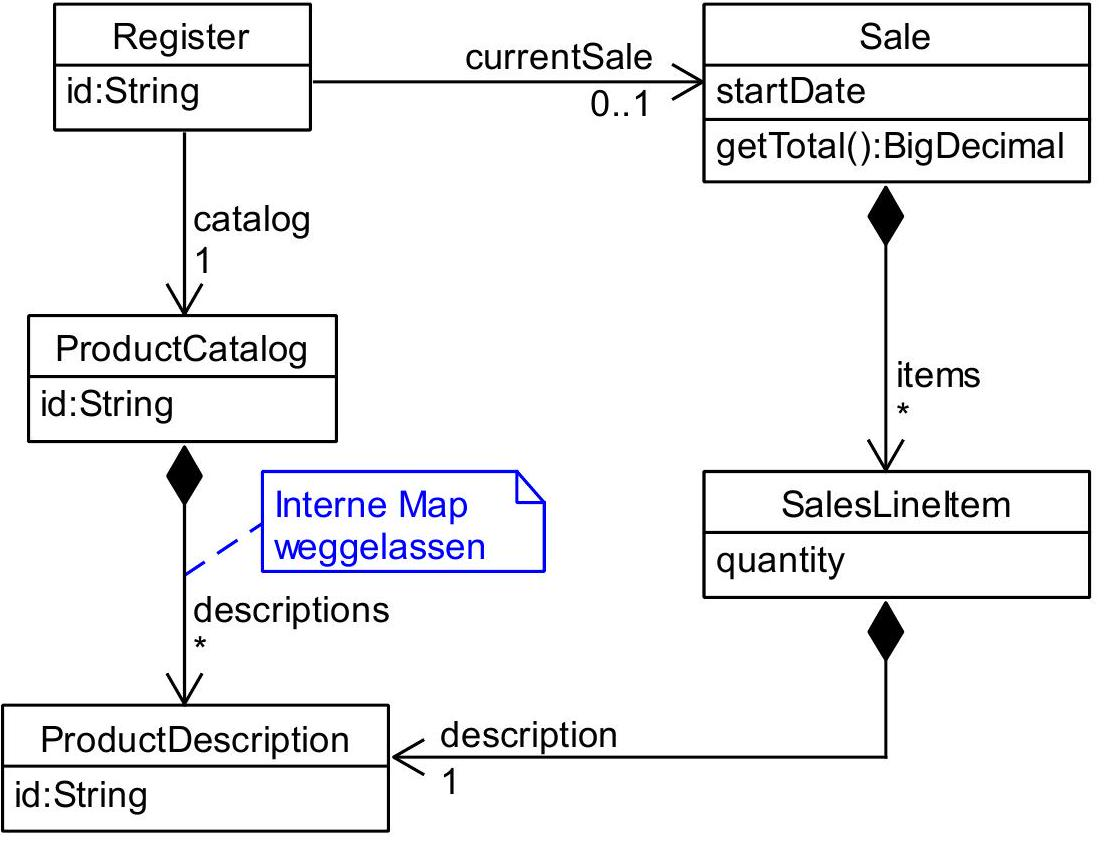
\includegraphics[width=\linewidth]{images/2025_01_02_1fd681d207513c8e8344g-27(1)}
\end{center}

\section*{Klassendiagramm Variante:}
\begin{center}
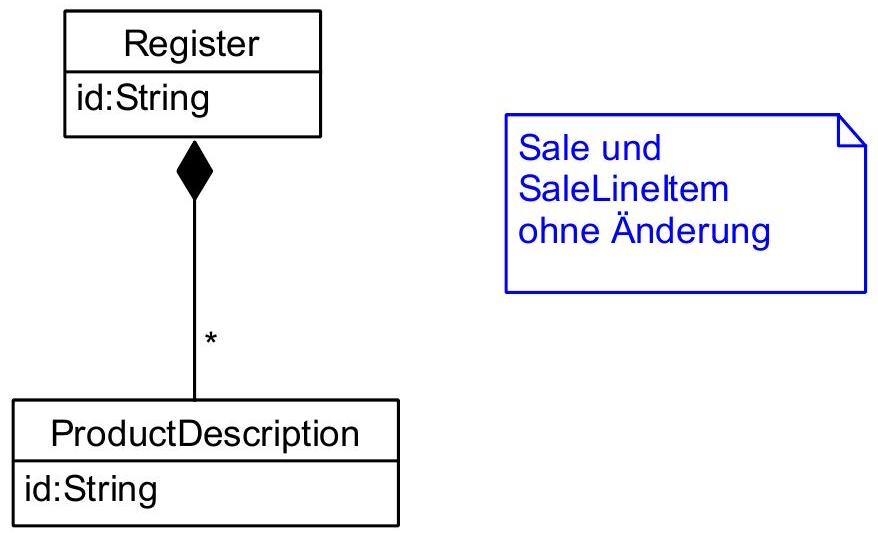
\includegraphics[width=\linewidth]{images/2025_01_02_1fd681d207513c8e8344g-27}
\end{center}

Warum braucht es ProductCatalog?

\begin{itemize}
  \item Es ginge natürlich auch ohne diese Klasse.
  \item Domänen-Orientierung und High Cohesion sprechen für diese Klasse.
  \item Controller nicht überladen!
\end{itemize}

\section*{Enterltem (3)}
School of Engineering InIT Institut für angewandt Informationstechnologie

\section*{1. Controller: Bereits definiert, nämlich Register}
\begin{enumerate}
  \setcounter{enumi}{1}
  \item Ziel: Neue Instanz von SalesLineltem
  \item Creator Pattern anwenden: Container von SalesLineltem soll diese erstellen, das wäre die Klasse Sale.
  \item Bedingt neue Methode in Sale, die neben dem Erstellen einer neuen Instanz von SalesLineltem, diese der internen Liste hinzufügt.
  \item Bei der Instanzierung von SalesLineltem können die Attributewerte «quantity» und «description» gleich als Parameter mitgegeben werden.\\
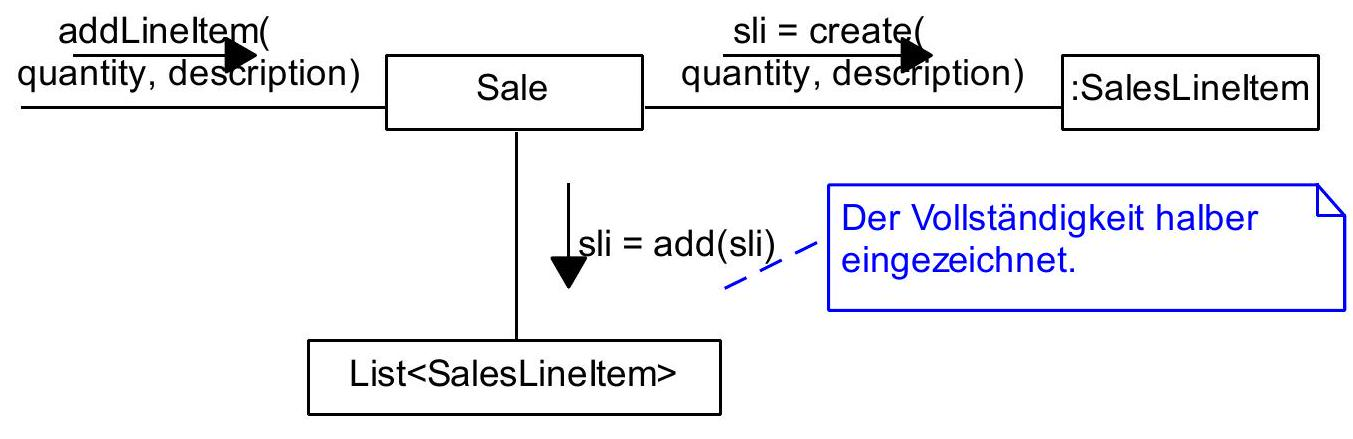
\includegraphics[width=\linewidth]{images/2025_01_02_1fd681d207513c8e8344g-28}
\end{enumerate}

\section*{Enterltem (4)}
School of

\section*{3. Weg zum Ziel:}
\begin{enumerate}
  \item Sale ist direkt von Register aus erreichbar, d.h. wir brauchen keine Zwischenstation.
  \item Allerdings wird in SaleLineltem eine Referenz auf ProductDescription benötigt, die über den Parameter itemId spezifiziert wird.
  \item Bevor wir Sale den Auftrag geben, eine neue Instanz von SaleLineltem zu erstellen, müssen wir über den ProductCatalog die itemId in die entsprechende ProductSpecification Instanz umwandeln.\\
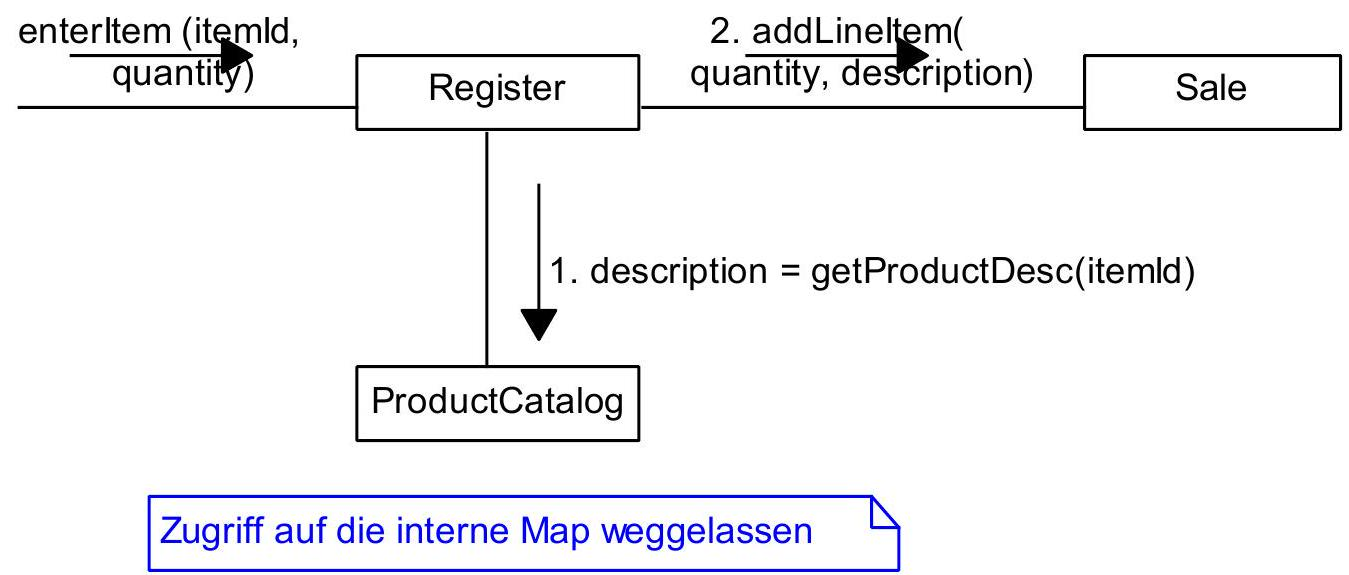
\includegraphics[width=\linewidth]{images/2025_01_02_1fd681d207513c8e8344g-29}
\end{enumerate}

\section*{4. Veränderungen programmieren: Bisherige Teile zusammenbauen}
\begin{center}
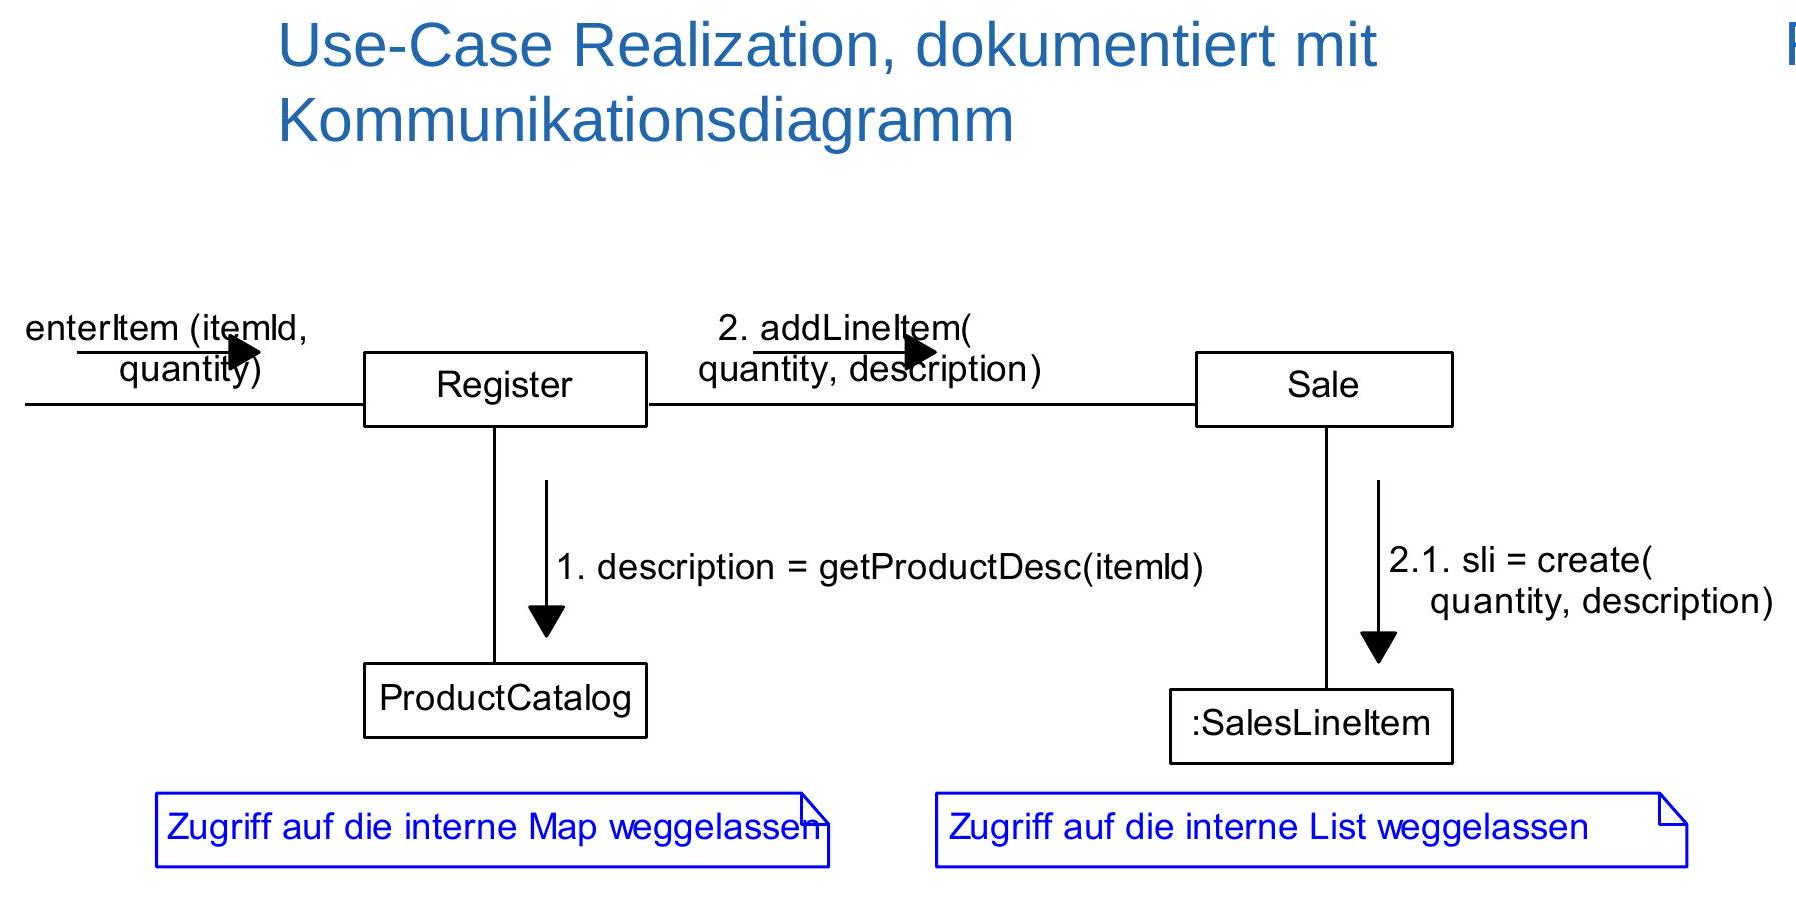
\includegraphics[width=\linewidth]{images/2025_01_02_1fd681d207513c8e8344g-30(1)}
\end{center}

Resultierendes DCD\\
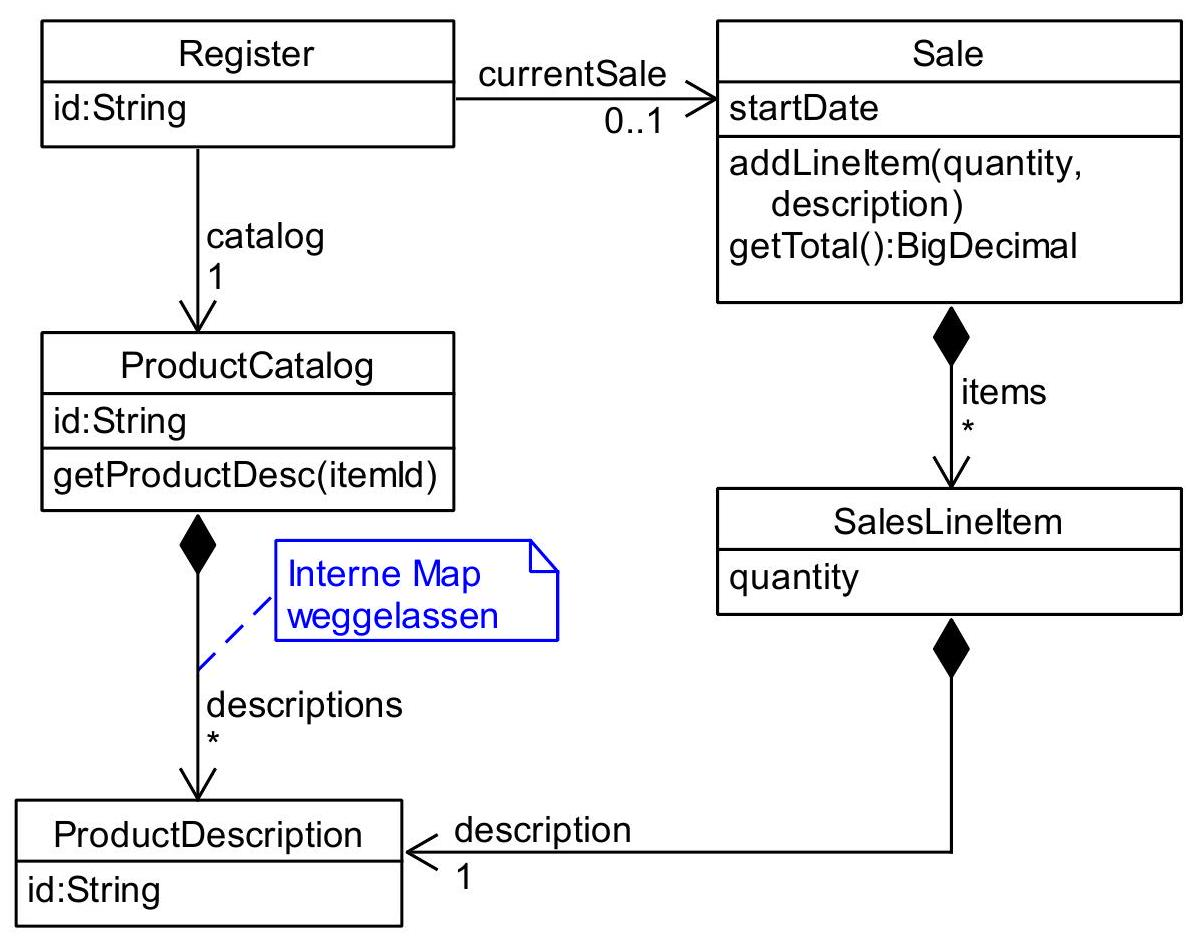
\includegraphics[width=\linewidth]{images/2025_01_02_1fd681d207513c8e8344g-30}

\section*{EndSale (1)}
School of

\section*{Vorbereitungsarbeiten}
\begin{enumerate}
  \item Use Case «Process Sale», fully dressed ausgearbeitet
  \item Systemoperation «endSale()
  \item Operation Contract, Nachbedingungen
\end{enumerate}

\begin{itemize}
  \item Aktuelle Sale-Instanz ist markiert als „abgeschlossen" (complete)
\end{itemize}

\begin{enumerate}
  \setcounter{enumi}{3}
  \item Aktueller Status der Software: Siehe vorhergehendes Beispiel
  \item Klassen Register, Sale erstellt
  \item Die bereits existierenden Software-Klassen genügen für diese Systemoperation.
\end{enumerate}

\section*{EndSale (2)}
School of

\begin{enumerate}
  \item Controller: Bereits definiert, nämlich Register
  \item Ziel: Sale als abgeschlossen markieren
  \item Sale ist direkt von Register aus erreichbar
  \item Sale erhält eine neue Methode: becomeComplete(). Im Moment setzt diese Methode nur ein boolean Attribute.\\
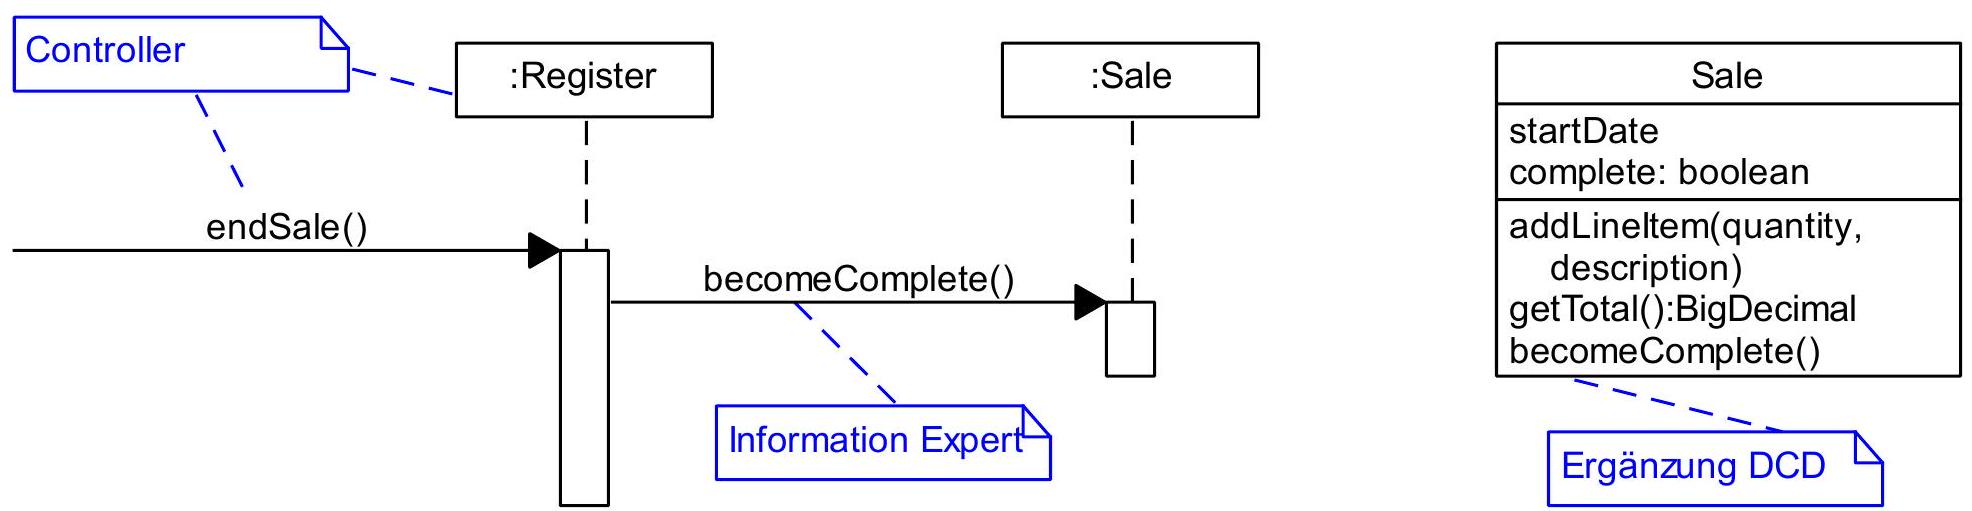
\includegraphics[width=\linewidth]{images/2025_01_02_1fd681d207513c8e8344g-32}
\end{enumerate}

\section*{GetTotal (1)}
\section*{Vorbereitungsarbeiten}
\begin{enumerate}
  \item Use Case «Process Sale», fully dressed ausgearbeitet
  \item Systemoperation «getTotal()»
  \item Operation Contract, Nachbedingungen
\end{enumerate}

\begin{itemize}
  \item Reine Abfrage, macht keine Veränderungen
\end{itemize}

\begin{enumerate}
  \setcounter{enumi}{3}
  \item Aktueller Status der Software: Siehe vorhergehendes Beispiel
  \item Klassen Register, Sale, SalesLineltem und ProductDescription vorhanden
  \item Die bereits existierenden Software-Klassen genügen für diese Systemoperation.
\end{enumerate}

\section*{GetTotal (2)}
\begin{enumerate}
  \item Controller: Bereits definiert, nämlich Register
  \item Ziel: Keine Veränderung, aber Rückgabewert zeigt den Gesamtbetrag der aktuellen Sale Instanz.
  \item Sale ist der Information Expert (GRASP) für diese Aufgabe und direkt von Register aus erreichbar
  \item Sale erhält eine neue Methode: getTotal(). Diese Verantwortlichkeit kann Sale aber nicht alleine wahrnehmen, es braucht noch SalesLineltem und ProductDescription dafür.\\
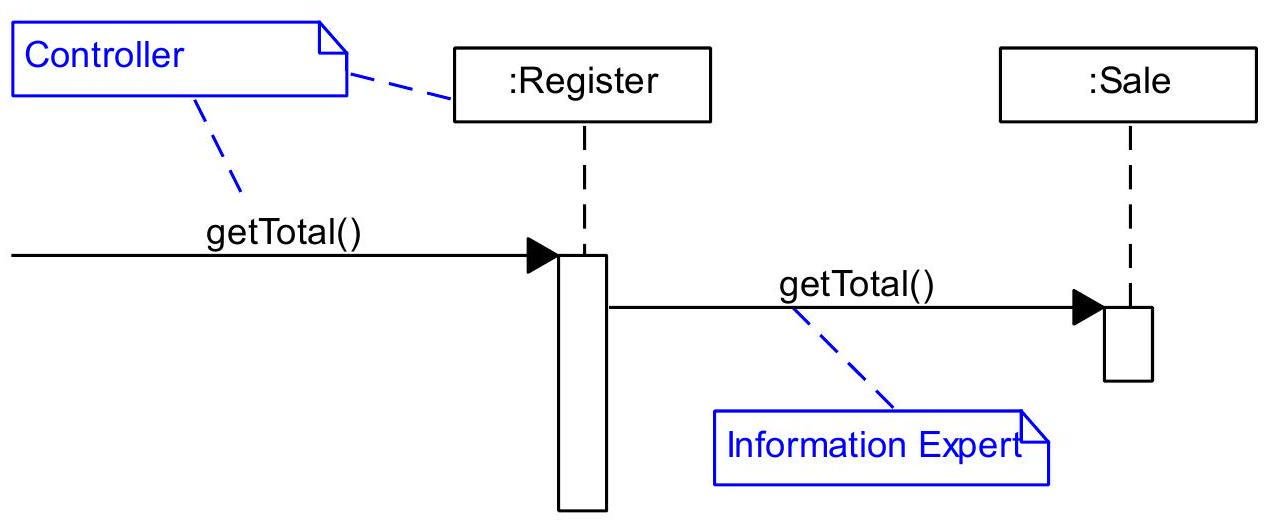
\includegraphics[width=\linewidth]{images/2025_01_02_1fd681d207513c8e8344g-34}
\end{enumerate}

\section*{GetTotal (3)}
School of Engineering\\
InIT Institut für angewandte Informationstechnologie\\
5. Sale muss nun das Zwischentotal seiner SalesLineltems zusammenzählen und zurückgeben.

\begin{itemize}
  \item Die Berechnung des Zwischentotals wird gemäss Information Expert an SalesLineltem delegiert. Dafür ruft diese die Methode getPrice() von ProductDescription auf.\\
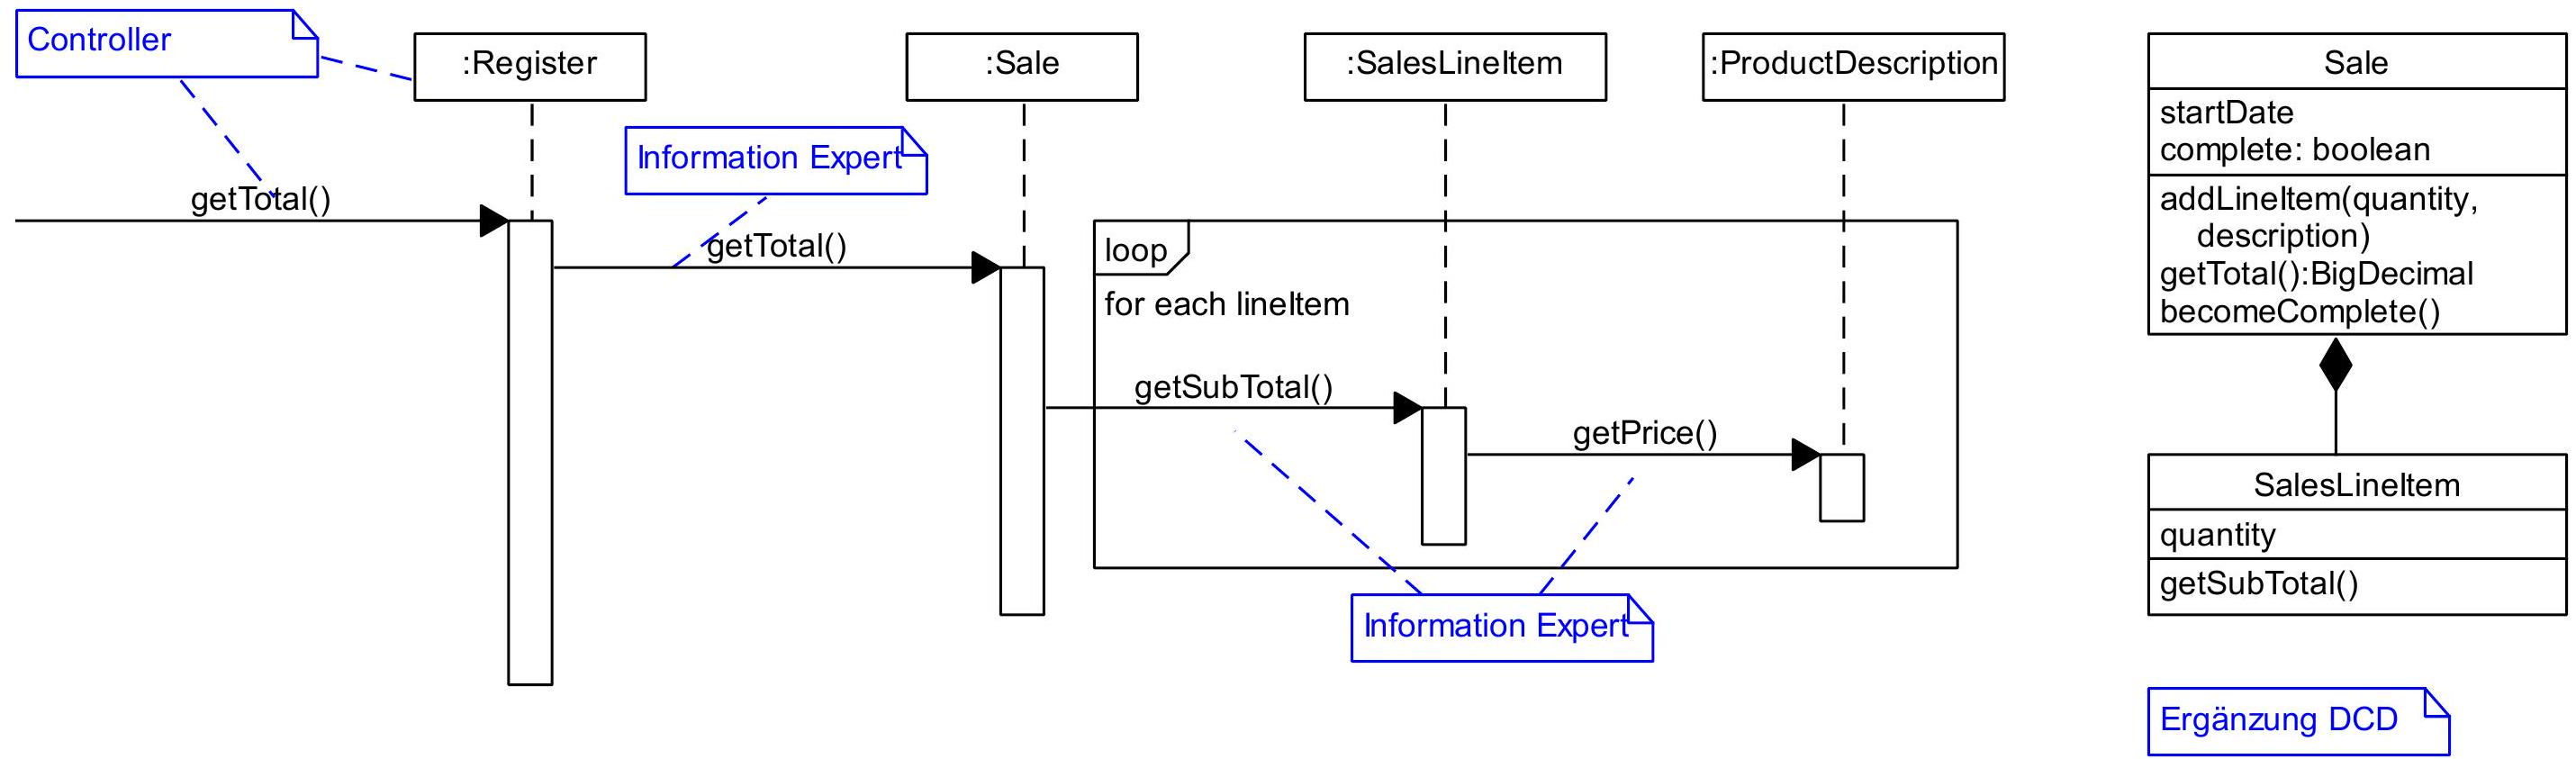
\includegraphics[width=\linewidth]{images/2025_01_02_1fd681d207513c8e8344g-35}
\end{itemize}

\section*{GetTotal (4)}
\begin{itemize}
  \item Wir betrachten nun alternative Lösungen und evaluieren sie gemäss Low Coupling und High Cohesion.
  \item In der folgenden Variante macht Sale alles selber. Es holt sich alle Daten aus SalesLineltem und ProductDescription und führt alle Berechnungen selber durch.
  \item Dadurch sinkt die Kohäsion von Sale und das Information Expert Pattern ist für SalesLineltem nicht mehr erfüll. Zusätzlich wird eine weitere Kopplung von Sale zu ProductDescription eingeführt.
  \item Fazit: Nicht empfehlenswert.\\
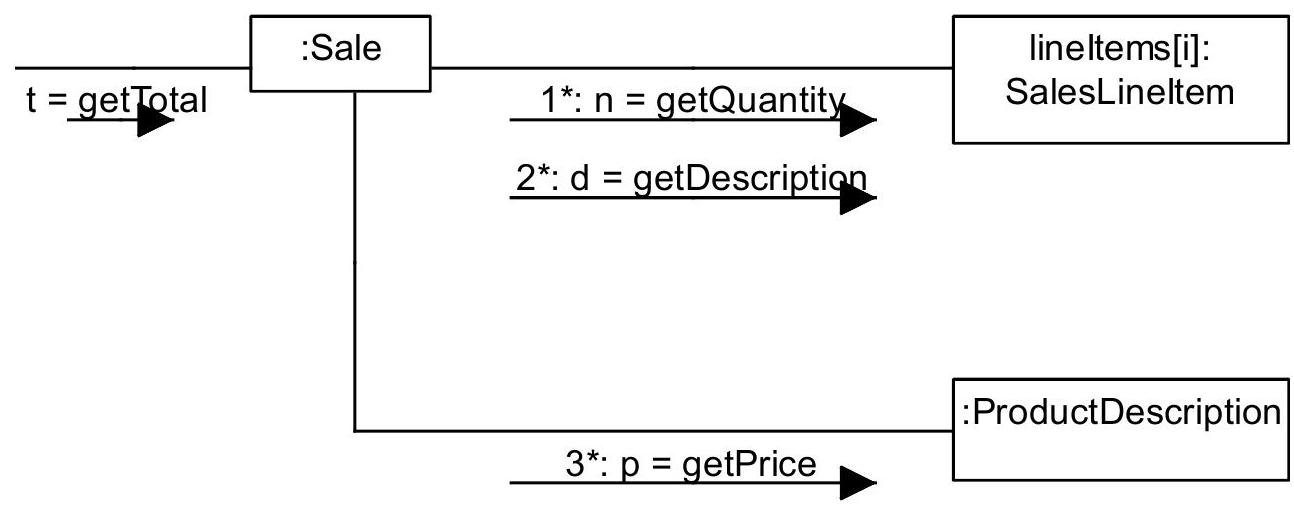
\includegraphics[width=\linewidth]{images/2025_01_02_1fd681d207513c8e8344g-36}
\end{itemize}

\section*{GetTotal (5)}
School of

\begin{itemize}
  \item In der folgenden Variante führen wir noch eine weitere Klasse SaleHandler ein, die alle Berechnungen ausführt.
  \item Das Information Expert Pattern ist für Sale und SalesLineltem nicht mehr erfüllt.
  \item Zusätzliche Klasse und zusätzliche Kopplungen.
  \item Fazit: Nicht empfehlenswert.\\
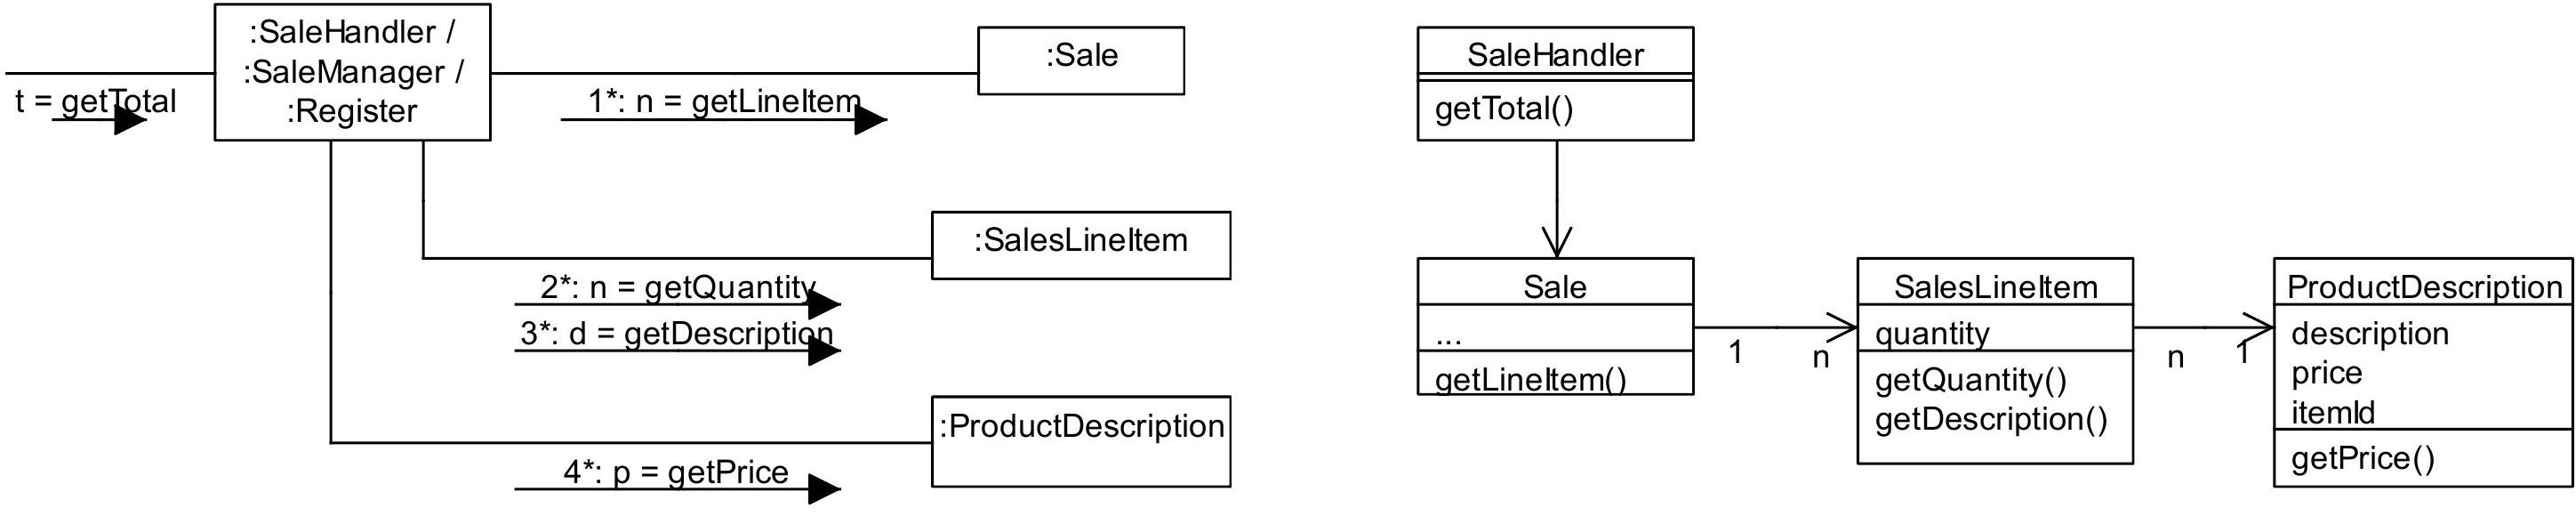
\includegraphics[width=\linewidth]{images/2025_01_02_1fd681d207513c8e8344g-37}
\end{itemize}

\section*{Vorbereitungsarbeiten}
\begin{enumerate}
  \item Use Case «Process Sale», fully dressed ausgearbeitet
  \item Systemoperation «makePayment()»
  \item Operation Contract, Nachbedingungen\\
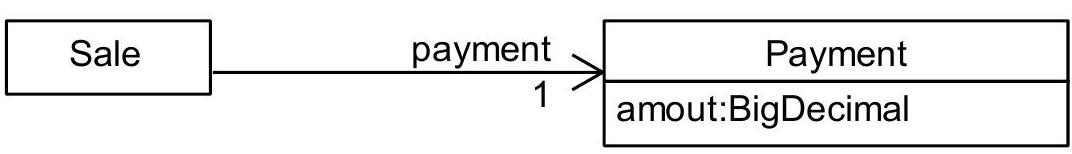
\includegraphics[width=\linewidth]{images/2025_01_02_1fd681d207513c8e8344g-38}
\end{enumerate}

\begin{itemize}
  \item Eine neue Instanz von Payment ist erzeugt und mit der aktuellen Instanz von Sale verknüpft.
\end{itemize}

\begin{enumerate}
  \setcounter{enumi}{3}
  \item Aktueller Status der Software: Siehe vorhergehendes Beispiel
  \item Klassen Register, Sale, SalesLineltem und ProductDescription vorhanden
  \item Wir brauchen eine Software-Klasse Payment, die wir aus dem Domänenmodell übernehmen können.
\end{enumerate}

\begin{itemize}
  \item Vielleicht erscheint es übertrieben, dafür eine eigene Software-Klasse mit nur einem Attribut zu erstellen.
  \item Die Orientierung an der Fachdomäne empfiehlt aber das Einführen auch „kleiner" Software Klassen, die aus der Fachdomäne inspiriert sind
  \item Die Bezahlung mit Cash ist eine Variante. In späteren Iterationen kommt die Bezahlung mit Kreditkarte hinzu.
\end{itemize}

\section*{MakePayment (2)}
School of

\begin{enumerate}
  \item Controller: Bereits definiert, nämlich Register
  \item Ziel: Neue Instanz von Payment, mit der aktuellen Instanz von Sale verknüpft.
  \item Payment ist über Sale von Register aus erreichbar.
  \item Wer erzeugt die neue Instanz von Payment?
  \item Creator Pattern anwenden: Sale ist nur bedingt der Container von Payment, arbeitet aber sehr eng damit zusammen.
  \item Wichtiger ist allerdings, dass alternative Varianten wegen Low Coupling schlechter abschneiden.\\
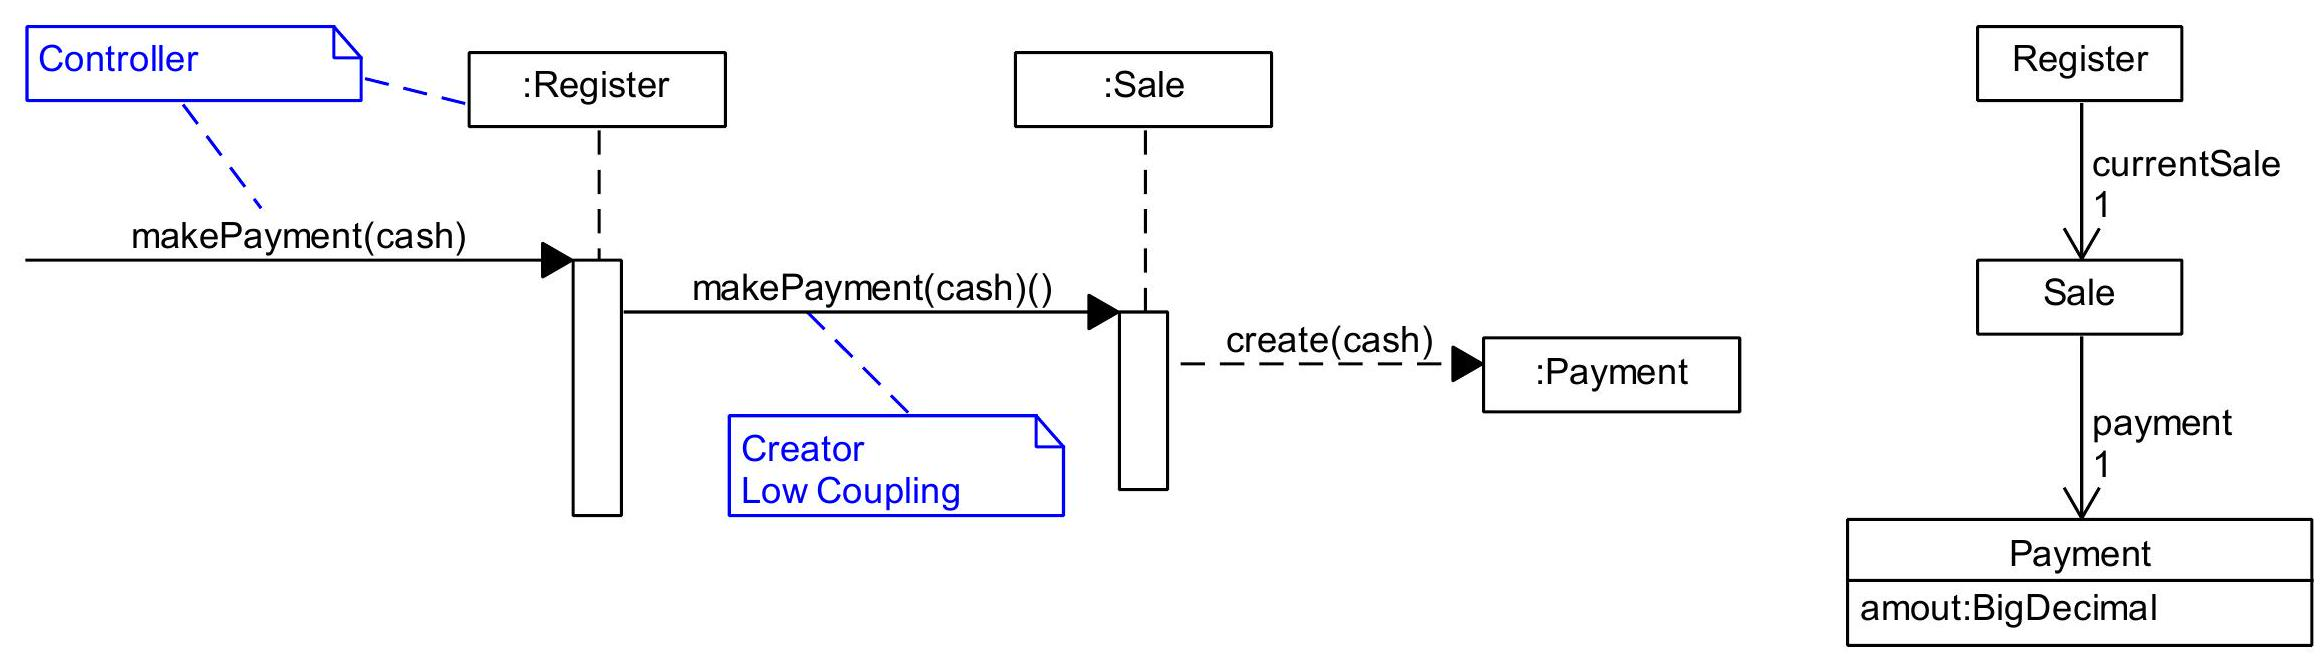
\includegraphics[width=\linewidth]{images/2025_01_02_1fd681d207513c8e8344g-39}
\end{enumerate}

\section*{MakePayment (3)}
School of

\section*{Alternative Lösung:}
\begin{itemize}
  \item Payment wird von Register erzeugt und an Sale übergeben.
  \item Dadurch wird eine neue Kopplung von Register auf Payment eingeführt, weshalb diese Lösung nicht empfehlenswert ist.\\
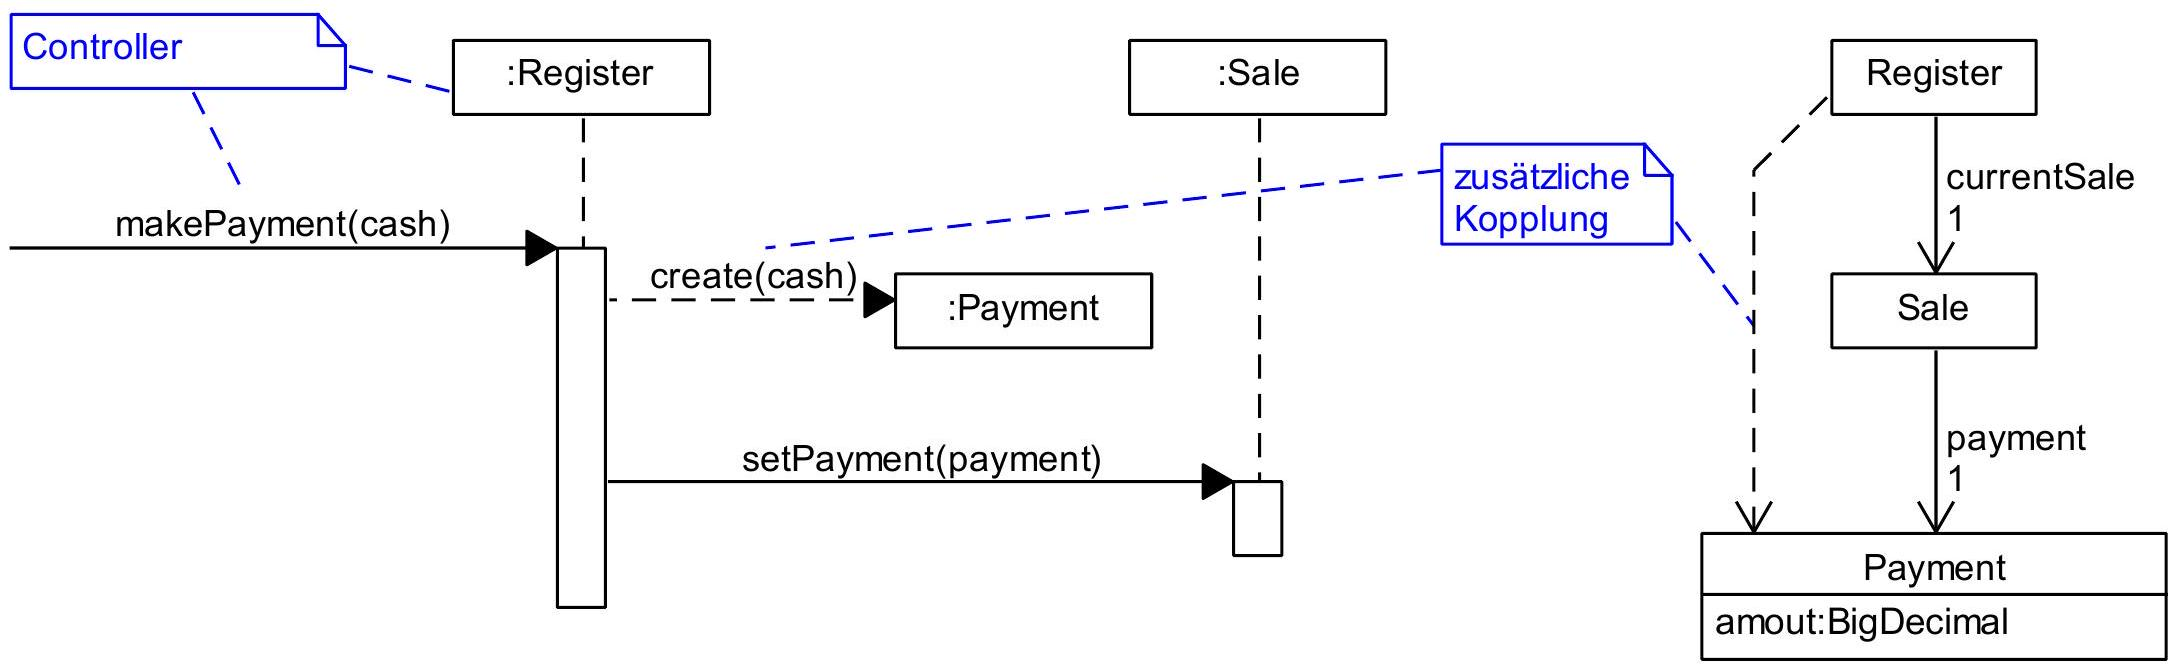
\includegraphics[width=\linewidth]{images/2025_01_02_1fd681d207513c8e8344g-40}
\end{itemize}

\begin{enumerate}
  \item Einfluss Analyse Artefakte
  \item UML und Design to Code
  \item Repetition GRASP
  \item Vorgehen
  \item Fallstudie «NextGenPos»
  \item Fallstudie «Monopoly»
  \item Wrap-up und Ausblick
\end{enumerate}

\begin{itemize}
  \item Wir führen nun die Use-Case Realization für die erste Iteration zur Entwicklung des Spiels „Monopoly" durch. Es ist ein weiteres Fallbeispiel aus Larman[1]
  \item In der ersten Iteration spielt der Computer „mit sich selber". Der Mensch beschränkt sich auf das Initialisieren und den Start des Spiels
  \item Die Systemoperation:
  \item initialize(numOfPlayers)
  \item playGame(idemId, quantity)
  \item Pro (künstlichem) Spieler muss zuerst mit 2 Würfeln gewürfelt werden, dann wird seine Spielfigur um die Anzahl Augen verschoben.
  \item In der ersten Iteration passiert noch nichts, wenn eine Figur auf einem Spielfeld landet.
\end{itemize}

\begin{enumerate}
  \item Einfluss Analyse Artefakte
  \item UML und Design to Code
  \item Repetition GRASP
  \item Vorgehen
  \item Fallstudie «NextGenPos»
  \item Fallstudie «Monopoly»
  \item Wrap-up und Ausblick
\end{enumerate}

\begin{itemize}
  \item Use-Case-Realization heisst die Tätigkeit, einen Use-Case zu realisieren, indem Software-Klassen Verantwortlichkeiten bis hin zum Code erhalten.
  \item Use-Case-Realization basiert auf den Analyse-Artefakten aus LE03 und LE04.
  \item Die Software Architektur gibt Vorgaben für die Umsetzung der Use-Cases.
  \item Die Anwendung der GRASP Prinzipien führt zu gutem, objektorientiertem und wartbarem Code.
  \item In der nächsten zwei Lerneinheiten werden wir:
  \item die GoF Design Patterns einführen und an vielen praktischen Beispielen anwenden.
\end{itemize}

\section*{Quellenverzeichnis}
[1] Larman, C.: UML 2 und Patterns angewendet, mitp Professional, 2005


\end{document}